%\documentclass{uai2025} % for initial submission
\documentclass[accepted]{uai2025} % after acceptance, for a revised version; 
% also before submission to see how the non-anonymous paper would look like 
                        
%% There is a class option to choose the math font
% \documentclass[mathfont=ptmx]{uai2025} % ptmx math instead of Computer
                                         % Modern (has noticeable issues)
% \documentclass[mathfont=newtx]{uai2025} % newtx fonts (improves upon
                                          % ptmx; less tested, no support)
% NOTE: Only keep *one* line above as appropriate, as it will be replaced
%       automatically for papers to be published. Do not make any other
%       change above this note for an accepted version.

%% Choose your variant of English; be consistent
\usepackage[american]{babel}
% \usepackage[british]{babel}

%% Some suggested packages, as needed:
\usepackage{natbib} % has a nice set of citation styles and commands
\bibliographystyle{plainnat}
\renewcommand{\bibsection}{\subsubsection*{References}}

% \usepackage{siunitx} % for proper typesetting of numbers and units


%% Provided macros
% \smaller: Because the class footnote size is essentially LaTeX's \small,
%           redefining \footnotesize, we provide the original \footnotesize
%           using this macro.
%           (Use only sparingly, e.g., in drawings, as it is quite small.)

%% Self-defined macros
\newcommand{\swap}[3][-]{#3#1#2} % just an example

% Language setup
\usepackage[american]{babel}

% Math and tables
\usepackage{mathtools} % Includes amsmath with improvements
\usepackage{booktabs} % For professional-quality tables
\usepackage{nicematrix}
\usepackage{bm} % Bold math symbols

% Diagrams and graphics
\usepackage{tikz}
\usetikzlibrary{
  positioning,
  bayesnet,
  fit,
  shapes.geometric,
  shapes,
  arrows.meta,
  calc
}
% TikZ styles
\tikzset{
  rounded box/.style={rectangle, rounded corners, draw, align=center, minimum height=1cm, minimum width=1.5cm},
  startstop/.style={rectangle, rounded corners, minimum width=3cm, minimum height=1cm, text centered, draw=black, fill=red!30},
  process/.style={rectangle, minimum width=3cm, minimum height=1cm, text centered, draw=black, fill=blue!30},
  decision/.style={diamond, minimum width=3cm, minimum height=1cm, text centered, draw=black, fill=green!30},
  arrow/.style={->,>=stealth},
  bidirected/.style={<->,>=stealth},
  dottededge/.style={dotted, thick}
}

% Miscellaneous packages
\usepackage{subcaption}
\usepackage[makeroom]{cancel}
\usepackage{centernot}
\usepackage{amsthm}
\usepackage{amssymb}
\usepackage{xfrac}
\usepackage[most]{tcolorbox}


% Theorem and definition styles
\theoremstyle{plain}
\newtheorem{theorem}{Theorem}
\newtheorem{lemma}{Lemma}
\newtheorem{proposition}{Proposition}
\newtheorem{observation}{Observation}
\newtheorem{corollary}{Corollary}[proposition]

\theoremstyle{definition}
\newtheorem{definition}{Definition}
\newtheorem{example}{Example}
\newtheorem{model}{Model}

\theoremstyle{remark}
\newtheorem{remark}{Remark}

% Self-defined macros
\newcommand{\dataset}{{\cal D}}
\newcommand{\fracpartial}[2]{\frac{\partial #1}{\partial #2}}
\newcommand{\ind}{\rotatebox[origin=c]{90}{$\models$}}
\newcommand{\notind}{{\centernot\ind_{\mathmakebox[5.7mm][r]{(T,\alpha)}}}}

% Bold symbols
\newcommand{\x}{{\mathbf{x}}}
\newcommand{\y}{{\mathbf{y}}}
\newcommand{\z}{{\mathbf{z}}}
\newcommand{\e}{{\mathbf{e}}}

% Sets and calligraphic letters
\newcommand{\Sset}{{\mathbf{S}}}
\newcommand{\lL}{{\mathbf{L}}}
\newcommand{\V}{{\mathbf{V}}}
\newcommand{\W}{{\mathbf{W}}}
\newcommand{\X}{{\mathbf{X}}}
\newcommand{\Y}{{\mathbf{Y}}}
\newcommand{\Z}{{\mathbf{Z}}}
\newcommand{\G}{{\mathcal{G}}}
\newcommand{\cG}{{\mathcal{G}}}
\newcommand{\cH}{{\mathcal{H}}}
\newcommand{\E}{{\mathcal{E}}}
\newcommand{\cE}{{\mathcal{E}}}
\newcommand{\cB}{{\mathcal{B}}}
\newcommand{\cD}{{\mathcal{D}}}
\newcommand{\cC}{{\mathcal{C}}}
\newcommand{\cM}{{\mathcal{M}}}
\newcommand{\cP}{{\mathcal{P}}}
\newcommand{\cS}{{\mathcal{S}}}
\newcommand{\cT}{{\mathcal{T}}}
\newcommand{\cU}{{\mathcal{U}}}
\newcommand{\cV}{{\mathcal{V}}}
\newcommand{\cW}{{\mathcal{W}}}

% Other mathematical notations
\newcommand{\MvO}{{\mathrm{MvO}}}
\newcommand{\Do}{{\mathrm{do}}}
\newcommand{\spr}{{\mathrm{spr}}}
\newcommand{\IP}{{\mathrm{IP}}}
\newcommand{\des}{{\mathrm{des}}}
\newcommand{\anc}{\mathrm{anc}}
\newcommand{\co}{\mathrm{co}}
\newcommand{\scc}{\mathrm{sc}}
\newcommand{\mic}{{\mathrm{mic}}}
\newcommand{\coh}{{\mathrm{coh}}}
\newcommand{\incoh}{{\mathrm{incoh}}}
\newcommand{\cohsc}{{\mathrm{cohscore}}}
\newcommand{\conditionedon}{\,|\,}

% Undirected edge macro
\newcommand{\undirectededge}[3][]{ %
  \foreach \x in {#2} { %
    \foreach \y in {#3} { %
      \path (\x) to [-, #1] (\y);
      \draw (\x) to (\y);
    }
  }
}


\title{Internal Incoherency Scores for Constraint-based Causal Discovery Algorithms}

% The standard author block has changed for UAI 2025 to provide
% more space for long author lists and allow for complex affiliations
%
% All author information is authomatically removed by the class for the
% anonymous submission version of your paper, so you can already add your
% information below.
%
% Add authors

\author[1]{\href{mailto:<jj@example.edu>?Subject=Your UAI 2025 paper}{Sofia Faltenbacher*}{}}
\author[2]{\href{mailto:<jj@example.edu>?Subject=Your UAI 2025 paper}{Jonas Wahl*}{}}
\author[1]{\href{mailto:<jj@example.edu>?Subject=Your UAI 2025 paper}{Rebecca Herman}}
\author[1]{\href{mailto:<jj@example.edu>?Subject=Your UAI 2025 paper}{Jakob Runge}}
% Add affiliations after the authors
\affil[1]{%
    Technical University Dresden
}
\affil[2]{%
    German Research Center for Artificial Intelligence (DFKI)
}

\affil[*]{%
    equal contribution
}

\begin{document}
\maketitle

\begin{abstract}
Causal discovery aims to infer causal graphs from observational or experimental data. Methods such as the popular PC algorithm are based on conditional independence testing and utilize enabling assumptions, such as the faithfulness assumption, for their inferences.
In practice, these assumptions, as well as the functional assumptions inherited from the chosen conditional independence test, are typically taken as a given and not further tested for their validity on the data.
In this work, we propose internal coherency scores that allow testing for assumption violations and finite sample errors, whenever detectable without requiring ground truth or further statistical tests. 
We provide a complete classification of erroneous results, including a distinction between detectable and undetectable errors, and prove that the detectable erroneous results can be measured by our scores. We illustrate our coherency scores on the PC algorithm with simulated and real-world datasets, and envision that testing for internal coherency can become a standard tool in applying constraint-based methods, much like a suite of tests is used to validate the assumptions of classical regression analysis.
\end{abstract}

\section{INTRODUCTION}
Causal discovery, also known as causal structure learning, is a highly active research field with new methods being published at almost every major machine learning conference (see \cite{zanga2022survey,assaad2022survey,brouillard2024landscape} for recent surveys on methods and applications). The field aims to provide tools for inferring qualitative cause-and-effect relationships from observational and experimental data while elucidating the assumptions that are needed to do so. One of the seminal causal discovery algorithms that inspired many others is the PC-algorithm \citep{spirtes1991algorithm}. Starting from a fully connected graph, the PC-algorithm sequentially executes statistical tests for conditional independence (CI), pruning the graph whenever an independence is found and choosing the next tests based on the current state of the graph. Finally, it uses previously tested or additional conditional independence statements to orient as many edges as possible. 

The correctness of the PC algorithm and its descendants, such as FCI \citep{spirtes2001anytime} and PCMCI \citep{runge_detecting_2019,runge_discovering_2020}, is typically proven for an idealized setting without statistical finite sample errors. In this setting, it is shown that the output is sound and maximally informative as long as the data generation process satisfies the mechanistic assumptions of the algorithm \citep{Spirtes2000}. But theoretical results on finite sample performance are much harder to prove and therefore rare (see \citep{kalisch2007estimating}). Assessments of finite sample performance are common using any of a variety of performance metrics \citep{tsamardinos_max-min_2006,henckel2024adjustment,wahl2024separationbased}, but these metrics usually require knowledge of the ground truth causal graph, limiting these evaluations to simulated data that may have exploitable unrealistic artifacts \citep{reisach_beware_2021}. In addition, it is often unclear how well real-world data conforms to the assumptions of causal discovery. As a consequence of statistical errors and assumption violations, PC-like methods may return an output graph with conspicuous inconsistencies, such as conflicting edge orientations where the algorithm attempted to orient the same edge in different directions at different points of the procedure. 

The earliest versions of PC-like algorithms imposed orientation-conflict resolution strategies implicitly; for example, the first pseudo-code of the PC and FCI algorithms by \cite{spirtes_causation_1993} is often implemented with an order-dependent last-come-last-orient implicit conflict resolution, for instance in the package causal-learn \cite{zheng2024causal}. Later versions offered explicit strategies.
%\cite{colombo_order-independent_2014} proposed order-invariant versions of the algorithm called PC-Stable and FCI-Stable, but that result in conflict resolutions that are definitively inconsistent with the data (cite more conversation later down). 
\cite{ramsey2016improving} used a conflict resolution strategy that prioritizes some conditional independencies over others by sorting the p-values. While such strategies force an algorithm to return a graph with fewer or no explicit orientation conflicts, they do not address the extent to which underlying assumption violations or finite sample errors affect the pruning of the graph or the overall correctness of the results. 

An existing approach which directly addresses this question is the reformulation of constraint-based causal discovery as an optimization problem based on Boolean satisfiability solvers \citep{hyttinen2014constraint}. It retains high accuracy under statistical errors, but the accuracy comes at the price of %\footnote{It performs $\sum_{i=0}^{n-2} \binom{n}{2}\binom{n-2}{i}=\frac{2^{n-3}n!}{n-2}$ conditional independence tests, where $n \in \mathbb{N}$ is the number of variables.} 
superexponential growth in computational cost as the number of variables increases. \cite{ramsey_adjacency-faithfulness_2006} proposed conservative-PC which executes additional statistical tests to find local ambiguities in the graph. \cite{colombo_order-independent_2014} suggested resolving these with a majority vote and explicitly marking any remaining orientation conflicts.

As finite sample errors and some degree of assumption violations are unavoidable for real-world data, there is a need to develop better tests for model plausibility and robustness of causal discovery methods in general and PC-like methods in particular. Such tests must not rely on an underlying ground truth that is unavailable for real data. In this article, we propose a class of plausibility checks tailored to PC-like algorithms. Importantly, our checks only make use of information that the algorithm has already gained, thus avoiding additional statistical testing or prediction. We then prove that our proposed check will detect any erroneous result that are theoretically detectable given the information gained in one run of a PC-like method.
%especially since the machine learning community wants to incorporate the ideas from causal inference for more explainability and trustworthyness, to which an analysis of the sensitivity of the algorithms to assumption violations statistical errors is essential.

More broadly, we examine manifestations of assumption violations and errors of PC-based algorithms. We have a closer look at the aforementioned orientation conflicts and observe that their presence implies that there is no graph of the graph type assumed by the algorithm (e.g., directed acyclic graphs for PC, maximal ancestral graphs for FCI) that can accommodate the conditional independencies measured by the algorithm. We illustrate in Section \ref{sec:class_and_dect} that if conflicts are present, there is no guarantee that even seemingly undisputed orientations in a method's output graph are correct. In the presence of conflicts, it is thus impossible to arrive at a valid method output without a strategy that prioritizes some test results above others. 

Even in graphs without explicit orientation conflicts and ambiguities, it is possible that some of the conditional (in)dependencies implied by the method's output graph contradict those that the algorithm has measured during its run. While a perfect match is often unachievable on finite-sample data, we argue that the degree of their mismatch provides valuable information on the correctness of statistical and mechanistic assumptions, and in Section \ref{sec:score} we propose scores that quantify this mismatch. In the absence of assumption violations and statistical errors, any sound algorithm will receive a coherency score of one. In the presence of assumption violations and statistical errors, a high score indicates that the output graph is a near-optimal representation of the CI test results while a low score indicates that the graph does not serve as a useful interpretation of the data.
%Further, we prove that the union of results with conflicts and results with incoherencies is exactly the subset of erroneous results which is detectable at all given the conditional independence test results and the output graph. 
We therefore argue that coherency scores are powerful tools to test the plausibility of method assumptions without access to the ground truth. Since explicit resolution of orientation conflicts or ambiguities always leads to incoherencies, different resolution strategies can lead to different incoherency scores, and these scores can in turn be used to find an optimal–-in the sense that it minimizes internal incoherencies–-resolution strategy.

This work is structured as follows. Section \ref{sec:preliminaries} introduces necessary notations and conventions. In Section \ref{sec:sources_detect}, we discuss and classify different types of errors and their consequences in PC-based causal discovery. We illustrate our classification through simple examples for different failure modes and prove that incoherencies capture all errors that are detectable without further information. In Section \ref{sec:score}, we define the coherency scores that are the central tool of this work. These scores are then applied to several toy examples, simulations, and the auto MPG real world data set \citep{auto_mpg_9} in Section \ref{sec:experiments}. Additional examples, experiments and proofs are summarized in the supplementary material.


%Together, by finding incoherencies, we can detect and quantify all erroneous results that are detectable given the information described above. Incoherencies can hint us at the fact that we are assuming linearity on nonlinear relationships, or that we assume causal sufficiency when there are hidden common causes.

%Not having to do additional tests as for satsolvers or conservative-PC comes with several advantages such as a better runtime and no risk for new statistical errors. The incoherency score we suggest is, however, also applicable to versions with additional tests. The trade-off between accuracy and runtime can therefore be configured by the user.

\paragraph{Related work}
While the PC algorithm and its variants remain among the most popular causal discovery tools, which is exactly why we believe improved error quantification is necessary, other independence test-based methods have been introduced as a response to some of the PC algorithm's shortcomings. In addition to the aforementioned Boolean satisfiability solvers \cite{hyttinen2013discovering,hyttinen2014constraint}, \cite{claassen_bayesian_2012} and \cite{jabbari2017discovery} combine CI testing with Bayesian approaches that provide a best fit to the tested constraints. In \citep[Appendix F]{wahl2024separationbased}, the difficulties connected to orientation conflicts are discussed in the context of distance metrics for causal graphs. 
For general causal discovery methods, different plausibility tests have been proposed in \cite{faller_self-compatibility_2023,eulig2023toward,schkoda2024cross}. These checks can be applied more broadly than ours, but they also require additional testing or several method runs on different sets of variables, while ours only uses information that the algorithm has already gained but is specific to PC-like methods. \cite{ramsey2024choosing} presented a test for whether the Markov condition holds or does not hold in DAGs and CPDAGs.

%\textcolor{blue}{@all: Is there other relevant related work?}

%\textcolor{blue}{@all Short overview of the structure of the paper neccessary?}

\section{PRELIMINARIES AND NOTATION} \label{sec:preliminaries}

In this work, $\X=(X^1, \dots , X^d)$ with $d \in \mathbb{N}$ denotes a set of nodes that represent random variables in a structural causal model (SCM) as defined by \cite{pearl_causality_2009}, and $\cG$ denotes a causal graph over $\X$. If the data generating process is a known SCM, the causal graph implied by this SCM is denoted by $\cG_{true}$. Causal graphs come with a notion of graphical \emph{separation} such as $d$-separation for directed acyclic graphs (DAGs, e.g. \cite{pearl_causality_2009}), $m$-separation for maximal ancestral graphs (MAGs, e.g. \citep{zhang_causal_2008}), and $\sigma$-separation for cyclic graphs (e.g. \citep{bongers_foundations_2021}). Unless indicated otherwise, statements in this work do not depend on the type of graph as long as one consistently uses the corresponding criterion for separation and its counterpart: \emph{connection}. We represent separation and connection statements with tuples consisting of two singular nodes and a (possibly empty) disjoint subset of nodes. The set of all such statements is denoted by
\begin{equation*}
    \cC=\left\{(X,Y,\Sset) \, \big| \, X,Y \in \X, \ X \neq Y, \Sset \subseteq \X \backslash\{X,Y \} \right\},
\end{equation*}
and given a causal graph $\cG$, the relevant notion of separation specifies for each tuple $(X,Y,\Sset)$ whether it is a \emph{separation statement} $X\bowtie_{\cG} Y\conditionedon \Sset$ ($X$ and $Y$ are separated given $\Sset$) or a \emph{connection statement} $X\centernot{\bowtie}_{\cG}Y \conditionedon \Sset$ ($X$ and $Y$ are connected given $\Sset$). We define the separation indicator function $\iota_{\cG}:\cC \to \{0,1 \}$ as $\iota_{\cG}(X,Y,\Sset)=1$ if $X \bowtie_{\cG} Y \conditionedon \Sset$ and as $\iota_{\cG}(X,Y,\Sset)=0$ otherwise.
%\begin{align*}
%    \iota_{\cG}(X,Y,\Sset) = \begin{cases} 1 \quad &\text{if } X \bowtie_{\cG} Y \conditionedon \Sset \\  0 \quad &\text{else}.  \end{cases}
%\end{align*}
The set of separations is denoted by
\begin{equation*}
    \cC^{sep}=\left\{(X,Y,\Sset) \in \cC \, \big| \, \iota_{\cG}(X,Y,\Sset)=1 \right\}.
\end{equation*}
and the set of connections by
\begin{equation*}
    \cC^{con}=\left\{(X,Y,\Sset) \in \cC \, \big| \, \iota_{\cG}(X,Y,\Sset)=0 \right\}.
\end{equation*}

In a causal graph, an \emph{unshielded triple} is a triple of nodes $(X,Y,Z)$ such that the outer nodes are adjacent to the middle node but not to each other. An unshielded triple is a \emph{collider} if the edges $(X,Y)$ and $(Y,Z)$ point towards $Y$ (e.g. $X \to Y \leftarrow Z$), otherwise the triple is called a \emph{non-collider}. 

Two causal graphs $\cG, \cH$ in the same graph class are \emph{Markov equivalent} if they share the same separations, i.e. $\cC^{sep}(\cG) = \cC^{sep}(\cH)$ or, equivalently, the same connections. We denote their Markov equivalence class (MEC) by $[\cG]=\{\cH\,\conditionedon\, \cH\sim_{\mathcal{M}} \cG\}.$
For DAGs, MECs can be represented by a Complete Partially Directed Acyclic Graph (CPDAG), and for MAGs, by a Partial Ancestral Graph (PAG). 

%and the set of triples with conditioning set of cardinality $k$ by
%\begin{equation*}
%    \cC^k=\left\{(X,Y,\Sset) \in \cC \, \big| %\, |\Sset|=k \right\}.
%\end{equation*}

A distribution $\mathcal{P}_{\X}$ over the variables $\X$ is called \emph{Markovian} on a causal graph $\cG$ or an equivalence class $[\cG]$ if the separation statements $X \bowtie_{\cG} Y \conditionedon \Sset$ imply the conditional dependencies $X \ind_{\mathcal{P}_{\X}} Y \conditionedon \Sset$ between the corresponding variables. It is called \emph{faithful} on $\cG$ if the conditional independencies $X \ind_{\mathcal{P}_{\X}} Y \conditionedon \Sset$ imply the separation statements for the corresponding nodes in $\cG$.

$\cM$  will be our symbol for a constraint-based causal discovery method. For example, $\cM$ could be a stand-in for variants of the PC algorithm like the classical PC or FCI algorithm (see, e.g. \cite{spirtes_causation_1993}), the PC-stable algorithm (see, e.g. \cite{colombo_order-independent_2014}), or the PCMCI algorithm family (see, e.g. \cite{runge2019inferring,runge_discovering_2020}). 

Let $( \x_1,\dots,\x_n ) \in \mathbb{R}^{(d \times n)}$ be $n \in \mathbb{N}$ samples drawn from the $d$-dimensional distribution $\mathcal{P}_{\X}$. Any constraint-based causal discovery method uses one or several statistical tests for conditional independence (CI), or dependence \citep{malinsky2024cautious} for which all statements can be formulated analogously. Let $T$ be a CI test and let $\alpha$ be the significance level. For brevity, we assume that the PC-like method uses only one type of CI test on all tested statements, but all results can be generalized in a straightforward way to algorithm variants using different types of tests. 

Common CI tests include Fisher's Z test for conditional independence in the linear Gaussian setting, kernel-based methods \citep{zhang2011kernel}, regression-based tests including the generalized covariance measure \citep{shahpeters}, or CMIknn \citep{runge2018conditional}, which is based on a nearest neighbour estimator of the conditional mutual information. 
%\textcolor{blue}{TODO: cite the corresponding paper for each test}

As we did for graphical separation, we now define a conditional independence test indicator function $\iota_{(T,\alpha)}:\cC \to \{0,1 \}$ for a CI test $(T,\alpha)$ as $\iota_{(T,\alpha)}(X,Y,\Sset) =1$ if $X \ind_{(T,\alpha)} Y \conditionedon \Sset$ (i.e. the tuple tested independent), and $\iota_{(T,\alpha)}(X,Y,\Sset) =0$ otherwise.
%\begin{align*}
% \iota_{(T,\alpha)}(X,Y,\Sset) = \begin{cases} 1 \quad &\text{if } X \ind_{(T,\alpha)} Y \conditionedon \Sset \\  0 \quad &\text{else}.  \end{cases}
%\end{align*}
By $\cT(\cM,T,\alpha) \subseteq \cC$ we denote the set of all statements that were tested during the execution of the algorithm $\cM$ using test $T$ at significance $\alpha$. We simply write $\cT$ if the referenced method, test, and threshold are clear from the context. 
%\begin{remark}
%    Unless all nodes are unconditionally and conditionally dependent on each other, $\cT$ is a proper subset of $\cC$ – this is what makes PC-like algorithms less computationally demanding than constraint-based alternatives like SATSOLVERS that test the whole set of all possible tuples $\cC$. The cardinality of $\cT$ for a given data set varies from one PC-like method to another.
%\end{remark}
The statements which tested conditionally independent (or for which dependence was rejected, e.g. in \citep{malinsky2024cautious}) are denoted by
\begin{equation*}
    \cT^{ind} = \left\{ (X,Y,\Sset) \in \cT  \,\big|\,  \iota_{(T,\alpha)}(X,Y,\Sset)=1\right\}.
\end{equation*}
The statements for which independence was rejected (or dependence was accepted) are denoted by 
\begin{equation*}
    \cT^{dep} = \left\{ (X,Y,\Sset) \in \cT \,\big|\,  \iota_{(T,\alpha)}(X,Y,\Sset)=0\right\}.
\end{equation*}

We call the the output graph $\cG_{out}$ of a PC-like method $\cM$ \textit{erroneous} if it is not Markov equivalent to $\cG_{true}$--the causal graph corresponding to the data generating SCM--or if there are marked conflicts or ambiguities in $\cG_{out}$ such that Markov equivalence is not well defined.


\section{SOURCES AND DETECTABILITY OF ERRONEOUS RESULTS} \label{sec:sources_detect}

This section lays the foundation for incoherency detection. We stress that the true causal graph $\cG_{true}$ is in general not known for real-world problems. The goal of this paper is to work out how to detect erroneous results without access to the ground truth whenever possible.

\subsection{SOURCES OF ERRONEOUS RESULTS} \label{sec:sources}

This subsection summarizes the various sources of error. We cluster the issues that can cause erroneous results into four error codes. This coding is complete in the sense that every assumption that could be violated is covered and finite sample issues are included. 

\textbf{E1: Faithfulness Violations.} Faithfulness is violated if $X \ind_{\cP_{\mathbf{X}}} Y \,|\, \textbf{S}$ but $(X,Y,\Sset)\notin\cC^{sep}$, i.e., if $X$ and $Y$ are conditionally independent given $\Sset$, but not separated given $\Sset$. Two examples of faithfulness violations due to counteractive mechanisms are discussed in Examples \ref{ex:unfaithfulness_detectable} and \ref{ex:unfaithfulness_undetectable}. 

\textbf{E2: Structural Violations.} Under this error code, we summarize all other violations of structural assumptions of PC-like algorithms, including acyclicity (which is assumed in all classical versions of PC, FCI and PCMCI+), causal sufficiency (e.g. in PC, PCMCI+) or causal stationarity (only for time series data, e.g. in PCMCI+). In other words, this error applies when the class of graphs considered by the algorithm is too limited, e.g. the class of DAGs cannot capture hidden confounding or cycles.

\textbf{E3: Conditional Independence Test Assumption Violations.} The assumptions of the conditional independence test $T$ might not hold in $\cP_{\mathbf{X}}$. This case covers violations of parametric or statistical assumptions such as linearity, additive noise, and the assumption that the samples are generated by independent, identically distributed variables. We also observe that nonlinear regression-based CI tests can be particularly tricky in the context of PC-like causal discovery, as the tests' assumptions on the functional relationship of regressor and regressand under the null might not be appropriate for every tested (in)dependence statement even if they match the functional relationship of a variable to its causes in the underlying SCM, as we illustrate in Appendix \ref{app:additional_examples}, Example \ref{ex.gpdc}. 

%\textcolor{blue}{add example from initial draft about a subtle CI test assumption violation here or in appendix.}

\textbf{E4: Finite Sample Errors.} Even if all assumptions of the CI tests hold, Type I and Type II errors are still expected on finite data. These errors lead to mistakenly retained or deleted edges and may influence edge orientations later on. Such errors can be due to unlucky draws from the underlying distribution. They can also be present in most simulations for certain unlucky causal structures. For example, for a fixed finite sample size, almost determinism may lead to wrong test results in most simulations (see Table \ref{tab:med_effect_four_nodes_10})  Figure \ref{fig:mediated_effect} in Appendix \ref{app:additional_experiments}.

\subsection{MANIFESTATIONS OF ERRONEOUS RESULTS}

When applying a PC-like method $\cM$ to real data, we typically do not know $\cG_{true}$, but only the tuples $\cT$ tested by the CI test $T$ with threshold $\alpha$, the corresponding test results, and the output graph $\cG_{out}$. From the latter, we can compute the value of $\iota_{\cG_{out}}(X,Y,\Sset)$ for any tuple $(X,Y,\Sset)$ when needed. 

We cluster the consequences of erroneous results on a distribution level into three cases.

\textbf{F1: There is no distribution $\cP_{\mathbf{X}}$ that can represent the observed conditional (in)dependence test results.} More formally, there is no $\cP_{\mathbf{X}}$ such that $(X,Y,\Sset) \in \cT^{ind}$ implies $X \ind_{\cP_{\mathbf{X}}} Y \,|\, \textbf{S}$ and $(X,Y,\Sset) \in \cT^{dep}$ implies $X \centernot{\ind}_{\cP_{\mathbf{X}}} Y \,|\, \textbf{S}$. This happens if the test results violate basic properties of conditional independence relations stated, for example, in \cite{pearl_causality_2009} as the \emph{graphoid axioms}.

\textbf{F2: A distribution $\cP_{\mathbf{X}}$ can represent the conditional independence test results, but none is Markovian and faithful to $\cG_{out}$.} In Example \ref{ex:unfaithfulness_detectable}, the distribution is neither Markovian and faithful to any DAG nor any MAG.

\textbf{F3: A distribution $\cP_{\mathbf{X}}$ can represent the conditional independence test results and is Markovian and faithful to $\cG_{out}$.} In Example \ref{ex:unfaithfulness_undetectable}, we show such an erroneous result for which the conditional independencies $\cT^{ind}$ are Markovian and faithful to $\cG_{out}$.

\paragraph{Orientation Conflicts}

If the assumptions of the PC algorithm, PC-stable, or PCMCI+ are perfectly satisfied, their output is a graph representing a Markov equivalence class, i.e. a CPDAG (PAGs for versions of FCI). As mentioned in the introduction, this is not always true in practice, as these algorithms may want to orient an edge in opposite directions due to conflicting CI test results, see Fig.~\ref{fig:orientation_conflicts} and Example \ref{ex:orientation_conflicts} below. This problem can be approached in two alternative ways; either by marking conflicts explicitly in the graph, or by forcing the algorithm to make a decision through a \emph{conflict-resolution strategy}, for instance by ranking tested conditional independencies by some heuristic such as the $p$-value \citep{ramsey2016improving}, or by allowing the algorithm to overwrite previous orientations. Clearly, these strategies have their own downsides, as overwriting makes the outcome depend on the variable order, while the relationship of $p$-values and test reliability can only serve as a heuristic due to the uniform distribution of the $p$-value under the null hypothesis \citep{ramsey2024choosing}. On the other hand, marking conflicts only where they appear may also be problematic. Example \ref{ex:orientation_conflicts} shows that in the presence of conflicts, even seemingly orientable edges may no longer be trustworthy. At the same time, the appearance of conflicts is valuable information as they are an indicator of assumption violations or finite sample issues, and when employing a conflict-resolution strategy, this information is no longer directly visible in the output graph. The coherency scores that we will introduce in Section \ref{sec:score} offer a middle ground and will be able to capture this information also after applying resolution strategies, so that it can be presented to the user.

\paragraph{Ambiguities} Some PC-like algorithms including conservative PC \citep{ramsey_adjacency-faithfulness_2006} and PC with the majority rule \citep{colombo_order-independent_2014} may additionally mark some unshielded triples as \emph{ambiguous}, indicating that the algorithm refuses to take a decision as to whether a triple is a collider or a non-collider. Ambiguities can be considered an honest version of marking conflicts as the algorithm explicitly indicates its uncertainty and does not base orientations on ambiguous triples (when using conservative PC) or picks the option for which there is more evidence and marks ambiguities in case of a tie (when applying the majority rule). Conflict-resolution strategies can also be applied to ambiguities and the to-be-defined coherency score accounts for them as well. 


We now define incoherent results of a PC-like method.
\begin{definition} \label{def:coherency}
  Let $\cM$ be a PC-like method using a CI test $(T,\alpha)$ with output $ \cG_{\mathrm{out}}$ without marked orientation conflicts or ambiguities. Let $\cT=\cT^{ind}\cup \cT^{dep}$ be the CI test results and $\cC^{sep}$ and $\cC^{con}$ the conditionally separated or connected tuples in $\cG_{\mathrm{out}}$. We call the result of the PC-like algorithm \textit{incoherent} if $\cT^{ind} \centernot{\subseteq} \cC^{sep}$ or $\cT^{dep} \centernot{\subseteq} \cC^{con}$.
\end{definition}
Note that testing for incoherencies is a straightforward task: The results of the CI tests can be saved while performing the method, and separation queries can be answered for all common graph types that are outputs of PC-like algorithms such as CPDAGs and MAGs after potentially resolving marked conflicts and ambiguities. For d-separation queries in CPDAGs and m-separation queries in MAGs, see, e.g. \cite{perkovic2015complete}.

The output of a PC-like method belongs to one of the following three categories.

\textbf{G1: Orientation conflicts or ambiguities are marked in $\cG_{out}$.} 
%We have discussed the consequences of orientation conflicts for other oriented edges in the graph in Example \ref{ex:orientation_conflicts}.

\textbf{G2: No conflicts or ambiguities are marked in $\cG_{out}$, but the results of the PC-like method are incoherent.} Example \ref{ex:unfaithfulness_detectable} shows a faithfulness violation (E1) that leads to no conflicts but incoherent results.

\textbf{G3: No conflicts or ambiguities are marked in $\cG_{out}$ and the results of the PC-like method are coherent.} Example \ref{ex:unfaithfulness_undetectable} shows a faithfulness violation (E1) that leads to such an erroneous result without conflicts or incoherencies.

\subsection{CLASSIFICATION AND DETECTION OF ERRONEOUS RESULTS} \label{sec:class_and_dect}

We demonstrate important observations with concrete examples leading up the main results about classification and detection of erroneous results. We start with the aforementioned Example \ref{ex:orientation_conflicts} that stresses how orientation conflicts not only reflect local, but global unreliability of the orientations. 

\begin{example} \label{ex:orientation_conflicts}
We consider the PC algorithm without any conflict resolution and the graph in Figure \ref{fig:orientation_conflicts}. We assume that the algorithm has found the colliders $W_1 \rightarrow X_3 \leftarrow W_2$ and $W_3 \rightarrow X_4 \leftarrow W_4$, all other unshielded triples have been classified as non-colliders. According to PC's orientation rules applied to the first collider, all edges between $X_3$ and $X_6$ have to be directed to the right. On the other hand, applying the same rule to the second collider directs these edges to the left, resulting in a conflict which is flagged at one or more of these edges (depending on the implementation). The edges left of $W_1 \rightarrow X_3 \leftarrow W_2$ are not flagged as the orientation rule that directs them away from the collider can be executed without conflicts. However, we argue that there is no reason to believe that even these orientations are still correct. After all, the underlying reason of the conflict is that there exists no DAG with the depicted skeleton for which the set of unshielded colliders is exactly $\{W_1 \rightarrow X_3 \leftarrow W_2, W_3 \rightarrow X_4 \leftarrow W_4 \}$, so we cannot trust the edges oriented because of them.
%\textcolor{blue}{@Jonas can formulate this better, to be finished}
%According to the following orientation rules, the unshielded non-colliders are then oriented. Starting from the left, two edges would be oriented to the right, ending at an orientation conflict as $X_3 \rightarrow X_4 \leftarrow W_3$ is to be oriented as a non-collider but would then be a collider. Analougously, starting at the right, two edges would be oriented to the left, arriving at an orientation conflict at the right. For a different order, the conflict can also appear at the edge in the middle and the right edge is oriented to the left and the left edge to the right. Depending on the order, edges without orientation conflicts are oriented differently which shows that also orientations without an orientation conflict can be affected from the consequences of an orientation conflict.
\end{example}

\begin{figure}[h]
    \centering
    \resizebox{0.4\textwidth}{!}{
        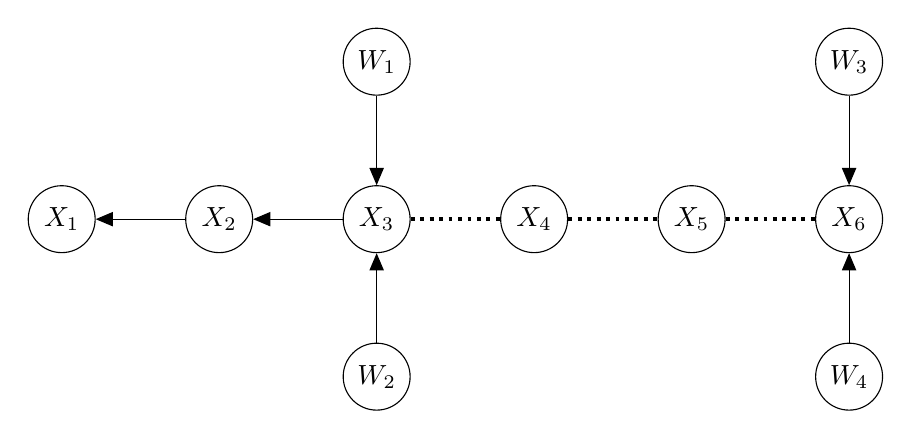
\begin{tikzpicture}[latent/.append style={minimum size=0.85cm}, obs/.append style={minimum size=0.85cm}, det/.append style={minimum size=1.15cm}, wrap/.append style={inner sep=2pt}, on grid]
            % Nodes
            \node[latent] (x) {$X_1$};
            \node[latent, right=2cm of x] (x2) {$X_2$};
            \node[latent, right=2cm of x2] (x3) {$X_3$};
            \node[latent, right=2cm of x3] (x4) {$X_4$};
            \node[latent, right=2cm of x4] (x5) {$X_5$};
            \node[latent, right=2cm of x5] (x6) {$X_6$};
            
            \node[latent, above=2cm of x3] (w1) {$W_1$};
            \node[latent, below=2cm of x3] (w2) {$W_2$};
            \node[latent, above=2cm of x6] (w3) {$W_3$};
            \node[latent, below=2cm of x6] (w4) {$W_4$};

            % Directed edges
            \draw[->] (w1) -- (x3);
            \draw[->] (w2) -- (x3);
            \draw[->] (w3) -- (x6);
            \draw[->] (w4) -- (x6);

            \draw[->] (x3) -- (x2);
            \draw[->] (x2) -- (x);

            % Dotted undirected edges
            \draw[dotted, line width=0.5mm] (x3) -- (x4);
            \draw[dotted, line width=0.5mm] (x4) -- (x5);
            \draw[dotted, line width=0.5mm] (x5) -- (x6);
        \end{tikzpicture}
    }
\caption{Without conflict resolution, only the dotted edges are marked as orientation conflicts, while also the seemingly orientable edges are no longer reliable.}
\label{fig:orientation_conflicts}
\end{figure}

Next is an example of a result without orientation conflicts which is incoherent.
\begin{example} \label{ex:unfaithfulness_detectable}
    We look at the following ground truth structural causal model:
    \begin{align*}
        X&=\eta_X,\,\,\,
        &Z&=X+\eta_Z, \\
        W&=Z+\eta_W, \,\,\,
        &Y&=2X-2W+\eta_Y;
    \end{align*}
    with independent, exogenous noise variables $\eta_X, \eta_Z, \eta_W, \eta_Y \sim \mathcal{N}(0,1)$. The corresponding true causal graph is $\cG_{true}$ in Figure \ref{fig:faithfulness_detectable}. As in Example \ref{ex:unfaithfulness_undetectable} there is a perfect counteractive mechanism (E1). Assuming no other sources of errors, this leads to the classical PC algorithm testing $\cT^{ind}=(X,Y,\emptyset), (Z,Y,\{X,W\}), (W,X,\{Z\})$ and all other tuples to be dependent.
    There is a distribution capturing these independencies and dependencies, but it is not Markovian and faithful to $\cG_{out}$ (F2). There are no orientation conflicts that arise while we perform the method, but we can detect that $X$ and $Y$ are tested conditionally independent, but they are not d-separated in $\cG_{out}$ (G2), see Figure \ref{fig:faithfulness_detectable}. Note that an undirected path in general does not imply d-connection, however $X$ and $Y$ are d-separated in this case as the path consists of undirected unshielded triples which fulfills the criterion for d-connection in CPDAGs which can for example be found in \cite{perkovic2015complete}. We can detect the incoherency using the scores that will be introduced in Section \ref{sec:score}.
\end{example}
Looking at the previous example, we can formulate the following observation.
\begin{observation} \label{obs:no_conflicts_but_detectable_errors}
    If the output of a PC-like algorithm has no conflicts, the result can still be incoherent.
\end{observation}
\begin{figure}[h]
    \centering
    \resizebox{.35\textwidth}{!}{ % Scale the entire figure uniformly
        \begin{tabular}{@{}c@{\hspace{1cm}}c@{}} % Added horizontal space between columns
            % First graph: G_true
            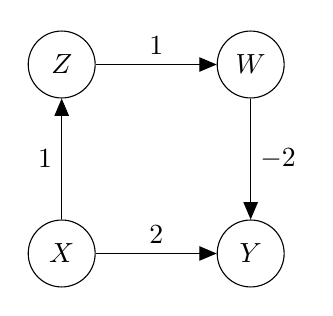
\begin{tikzpicture}[latent/.append style={minimum size=0.85cm}, obs/.append style={minimum size=0.85cm}, det/.append style={minimum size=1.15cm}, wrap/.append style={inner sep=2pt}, on grid]
                % Nodes
                \node[latent] (x) at (0,0) {$X$};
                \node[latent] (y) at (2.4,0) {$Y$};
                \node[latent] (z) at (0,2.4) {$Z$};
                \node[latent] (w) at (2.4,2.4) {$W$};
                
                % Edges with weights
                \draw[->] (x) -- (y) node[midway, above] {$2$};
                \draw[->] (x) -- (z) node[midway, left] {$1$};
                \draw[->] (z) -- (w) node[midway, above] {$1$};
                \draw[->] (w) -- (y) node[midway, right] {$-2$};
            \end{tikzpicture}
            &
            % Second graph: G_out
            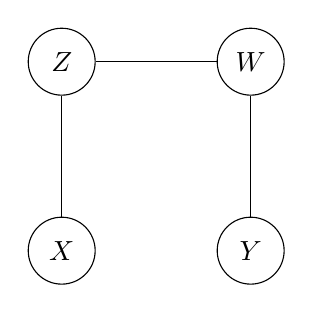
\begin{tikzpicture}[latent/.append style={minimum size=0.85cm}, obs/.append style={minimum size=0.85cm}, det/.append style={minimum size=1.15cm}, wrap/.append style={inner sep=2pt}, on grid]
                % Nodes
                \node[latent] (x) at (0,0) {$X$};
                \node[latent] (y) at (2.4,0) {$Y$};
                \node[latent] (z) at (0,2.4) {$Z$};
                \node[latent] (w) at (2.4,2.4) {$W$};
                
                % Undirected edges without weights
                \draw[-] (x) -- (z);
                \draw[-] (z) -- (w);
                \draw[-] (w) -- (y);
            \end{tikzpicture}
            \\
            $ \cG_{true} $ & $ \cG_{out} $
        \end{tabular}
    }
    \caption{Faithfulness violation leading to an incoherent erroneous result.}
    \label{fig:faithfulness_detectable}
\end{figure}

However, even checking for incoherencies is not sufficient to find all erroneous results as the next example shows.
\begin{example} \label{ex:very_small_effects_undetectable_erroneous}
    We look at the following ground truth structural causal model:
    \begin{equation*}
        X=\eta_X,\,\,\,\,\,
        Y=0.2\cdot X+\eta_Y,\,\,\,\,\,
        Z=0.2\cdot Y+\eta_Z,
    \end{equation*}
    with independent, exogenous noise variables $\eta_X, \eta_Y, \eta_Z \sim \mathcal{N}(0,1)$. The corresponding true causal graph is $\cG_{true}$ in Figure \ref{fig:very_small_effects_undetectable_erroneous}. Note that the total causal effect of $X$ on $Z$ is only $0.04$. Assuming no other sources of errors, fixing a sample size (e.g. 1000 samples), and choosing the classical PC algorithm as the PC-like method $\cM$, this leads to testing $X$ and $Z$ to be unconditionally independent (E4) in most simulations, see Section \ref{app:additional_experiments} in the Appendix. Note that the tuple $(X,Z,\{Y\})$ is not tested anymore as the edge between $X$ and $Z$ has already been removed. The only tuple tested conditionally independent is therefore $\cT^{ind}=(X,Y,\emptyset)$. There is a distribution capturing these independencies and dependencies which is also Markovian to $\cG^{out}$ (F3), see Figure \ref{fig:very_small_effects_undetectable_erroneous}. There are no orientation conflicts and the method has no internal incoherencies (G3). In this case, we have no chance to detect that in fact there was a finite sample error and out output is erroneous.
\end{example}

\begin{figure}[h]
    \centering
    \resizebox{.35\textwidth}{!}{ % Scale the entire figure uniformly
        \begin{tabular}{@{}c@{\hspace{1cm}}c@{}} % Added horizontal space between columns
            % First graph: G_true
            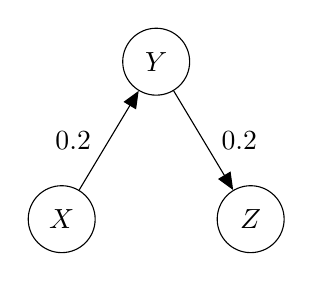
\begin{tikzpicture}[latent/.append style={minimum size=0.85cm}, obs/.append style={minimum size=0.85cm}, det/.append style={minimum size=1.15cm}, wrap/.append style={inner sep=2pt}, on grid]
                % Nodes
                \node[latent] (x) at (0,0) {$X$};
                \node[latent] (z) at (2.4,0) {$Z$};
                \node[latent] (y) at (1.2,2) {$Y$};
                
                % Edges with effects
                \draw[->] (x) -- (y) node[midway, left=3pt] {$0.2$};
                \draw[->] (y) -- (z) node[midway, right=3pt] {$0.2$};
            \end{tikzpicture}
            &
            % Second graph: G_out
            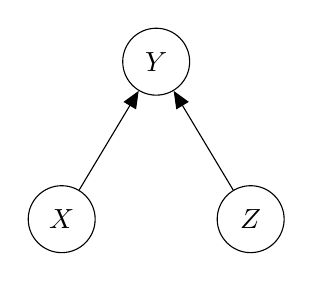
\begin{tikzpicture}[latent/.append style={minimum size=0.85cm}, obs/.append style={minimum size=0.85cm}, det/.append style={minimum size=1.15cm}, wrap/.append style={inner sep=2pt}, on grid]
                % Nodes
                \node[latent] (x) at (0,0) {$X$};
                \node[latent] (z) at (2.4,0) {$Z$};
                \node[latent] (y) at (1.2,2) {$Y$};
                
                % Edges for erroneous output
                \draw[->] (x) -- (y);
                \draw[->] (z) -- (y);
            \end{tikzpicture}
            \\
            $ \cG_{\text{true}} $ & $ \cG_{\text{out}} $
        \end{tabular}
    }
    \caption{Comparison of the true causal graph and an undetectable erroneous graph structure.}
    \label{fig:very_small_effects_undetectable_erroneous}
\end{figure}

The example illustrates the following observation.
\begin{observation} \label{obs:no_conflicts_but_errors}
    If the output of a PC-like algorithm has no conflicts and no incoherencies, the result can still be erroneous.
\end{observation}

The consequence of Observation \ref{obs:no_conflicts_but_errors} is that without access to the ground truth or doing additional tests, we cannot in general detect erroneous results of PC-like methods. In other words: There can be output graphs that are coherent but still wrong – and there is no chance to detect it without further effort. We formalize this property with the following definition.

\begin{definition}
    We call an erroneous result \textit{internally-detectable} if it can be detected by only accessing the results of the conditional independence tests for all tuples that were tested by the PC-like method $\cM$, i.e. $\cT^{ind} \cup \cT^{dep}$, as well as the output graph $\cG_{out}$ of $\cM$.
\end{definition}

The following proposition yields the exact subset of results for which this is the case. All proofs of the following results can be found in Section \ref{app:proofs} in the Appendix.

\begin{proposition}[Distributional Characterization of Internally-Detectable Erroneous Results] \label{prop:G3isF3}
    Erroneous results of a method $\cM$ are orientation-conflict-free and coherent with the CI test results $\cT^{ind} \cup \cT^{dep}$ (G3) if and only if there is a distribution that can represent the conditional independencies $\cT^{ind}$ and it is Markovian and faithful to $\G_{out}$ (F3).
\end{proposition}
We formulate a corollary which stresses why after resolving conflicts and ambiguities, the results stay internally-detectable as incoherecies.
\begin{corollary}[Resolved Conflicts and Ambiguities Imply Incoherencies] \label{cor:resolving}
    Resolving conflicts or ambiguities always leads to incoherencies.
\end{corollary}

\begin{remark}
    For the sake of completeness, we note that resolution strategies can lead to a resolved output graph that is incoherent given the CI test results–reflecting that there is no graph of the graph type assumed by the algorithm that matches all CI test results–but still Markov equivalent to the unknown true causal graph $\cG_{true}$. As a simple example, take an ambiguity resolution that ignores the one incorrect CI test result.
\end{remark}

\begin{proposition}[Graphical Characterization of Internally-Detectable Erroneous Results] \label{prop:detectable_graph}
    The internally-detectable erroneous results of a PC-like method $\cM$ is the union of results with marked conflicts or ambiguities and results with incoherencies.
\end{proposition}

Combining Corollary \ref{cor:resolving} and Proposition \ref{prop:detectable_graph} yields that after resolving all conflicts and ambiguities in output graphs, the internally-detectable erroneous results are exactly the ones with incoherencies. 

We have now stressed why detecting incoherencies is exhaustive to find internally-detectable erroneous results. Next, we show how to compute a score which not only detects them, but also quantifies different kinds of incoherencies which indicate in which way the result is flawed.

\section{QUANTIFYING INTERNAL COHERENCY}  \label{sec:score}

%We have proven that given the CI test results and the output graph, we cannot find all erroneous results of a PC-like method. The subset of erroneous results that we can detect is the ones with ambiguities, conflicts and incoherencies, or, for graphs in which all amiguities and conflicts have been resolved, simply all incoherent results. 
In this section, we quantify the overall incoherencies of a method by introducing three coherency scores. A high score represents a good performance. To define these scores, we distinguish two different kinds of incoherent tuples given the output graph and the conditional independence tests performed within the PC-like method of choice.

\begin{definition}
    A \textit{Markov incoherent} tuple $(X,Y,\mathbf{S})$ is in $\cC^{sep}$ and in $\cT^{dep}$, i.e. a tuple that has been tested dependent, but is separated in the output graph.
\end{definition}

\begin{definition}
    A \textit{faithfulness incoherent} tuple $(X,Y,\mathbf{S})$ is in $\cC^{con}$ and in $\cT^{ind}$, i.e. a tuple that has been tested independent but is connected in the output graph.
\end{definition}

Markov incoherent tuples may for instance appear because an edge has been deleted from a path connecting two nodes that were tested dependent. Conversely, a faithfulness incoherent tuple can be the result of an edge orientation that leaves a path open between nodes that were tested independent. As separations in the output graph are often considered more consequential for practitioners, Markov incoherencies may be particularly worrisome.

We now define the coherency score. Let $\cM$ be a PC-like method using a test $T$ with threshold $\alpha$. Let $w: \cT \rightarrow \mathbb{R}_{+}$ be a non-trivial weight function.

\begin{definition}
    Let $\cM$ be a PC-like method using a test $T$ with threshold $\alpha$. Let $w: \cT \rightarrow [0,\infty)$ be a non-trivial weight function. The \textit{total coherency score} is defined as
\begin{equation*}
    sc(w,\cM) = 1-\frac{\sum_{(X,Y,\mathbf{S}) \in \cT} w(X,Y,\mathbf{S})  \iota(X,Y,\mathbf{S})}{\sum_{(X,Y,\textbf{S}) \in \cT} w(X,Y,\mathbf{S}) },
\end{equation*}
where $\iota(X,Y,\mathbf{S})=|\iota_{\cG}(X,Y, \mathbf{S}) - \iota_{(T,\alpha)}(X,Y,\mathbf{S})|$.
\end{definition}

Different weight functions define different scores, see Appendix \ref{app:additional_scores}. Some natural weight function choices are:
\begin{itemize}
    \item \textbf{Standard Total Coherency Score}: For $w(X,Y,\mathbf{S})=1$, the coherency score simplifies to the total coherency rates.
    \item \textbf{Faithfulness Coherency Score}: Setting $w(X,Y,\Sset)=0$ for $(X,Y,\Sset) \in \cT^{dep}$ yields the faithfulness coherency score. (Setting $w(X,Y,\mathbf{S})=1$ for all other tuples, i.e. $(X,Y,\Sset) \in \cT^{ind}$, yields the standard faithfulness coherency score.)
    \item \textbf{Markov Coherency Score}: Setting $w(X,Y,\Sset)=0$ for $(X,Y,\Sset) \in \cC^{con}$ yields the Markov coherency score. (Setting $w(X,Y,\mathbf{S})=1$ for all other tuples, i.e. $(X,Y,\Sset) \in \cC^{sep}$, yields the standard Markov coherency score.)
    \item \textbf{Conditioning-Set-Size-Adjusted Score}: Choosing $w(X,Y,\Sset)=\exp(-|\mathbf{S}|)$ is a strictly decreasing weight function of the cardinality of the conditioning set and places more weight on incoherencies that occur for small conditioning sets.
\end{itemize}
The faithfulness and Markov coherency score and the conditioning-set-size-adjusted score can be combined. Further weight functions and combinations are explicitely written down in the Appendix in Section \ref{app:additional_scores}.


\section{EXPERIMENTS} \label{sec:experiments}

For all following experiments, we choose $\cM$ as the classical PC algorithm \citep{spirtes_causation_1993}. We choose the conditional independence test $T$ to be Fisher's Z test with threshold $\alpha=0.05$, and apply the methods to simulated as well as real-world data.

We first show how different assumption violations and finite sample errors affect the coherency scores on simulated data. We begin by evaluating the finite sample properties of common causal structures when only finite sample issues are present and continue with isolating different assumption violations to measure their impact. Eventually, we compute the score on the Auto MPG data set \citep{auto_mpg_9} on which PC in the stated configuration is applied in the causal-learn repository \citep{zheng2024causal}, and show in which ways the results are incoherent on this data set. 

\begin{figure}[h]
    \centering
    \includegraphics[width=0.85\linewidth]{figures/five_nodes.png}
    \caption{Small sample analysis for classical toy model}
    \label{fig:five_nodes}
\end{figure}

\textbf{Finite sample errors for common toy model} We examine data generated by SCMs of the following form:
\begin{align*}
   X &= \eta_{X}, &Y &= \eta_{Y}, &Z &= X+Y+\eta_{Z} \\
    W &= Z + \eta_{W}, &V &= Z +\eta_{V},
\end{align*}
where $\eta_{X},\eta_{Y},\eta_{Z},\eta_{V},\eta_{W} \sim \mathcal{N}(0,1)$ are independent, exogenous noise terms. Incoherencies on this toy model will only be caused by finite sample errors (E4) as the assumptions are fulfilled by design. To compute the average scores, we take the average of 100 repetitions. In Figure \ref{fig:five_nodes} we compare the average standard total (blue), faithfulness (orange), and Markov (green) coherency scores for SCMs of this form at different sample sizes (x axis, logarithmic scale). We observe that the result has a high coherency score from a sample size of 300 and a very high coherency scores from a sample size of 1000. In Section \ref{app:additional_experiments} of the Appendix, we examine the same model with different effect strengths. We also include extended tables including the standard deviation of the scores and the average number of orientation conflicts. In addition, we computed the average scores for different sample and effect sizes for other causal structures that are frequently analyzed.

% \begin{figure}
%     \centering
%     \includegraphics[width=1\linewidth]{uai2025-template/figures/mediated_effect.png}
%     \caption{Small sample analysis for mediated effect}
%     \label{fig:mediated_effect}
% \end{figure}

\textbf{Assumption violations} We generate data sets from the SCM in Example \ref{ex:unfaithfulness_detectable} and compute the average standard total, Markov and faithfulness coherency score in the presence of E1 errors. In almost all simulations, the detectable faithfulness violation leads to one faithfulness incoherent tuple $(X,Y,\emptyset)$ and one Markov incoherent tuple $(X,Y,\{W\})$. In contrast to the previous example, where increasing the sample size reduced sampling errors and incoherencies, the average score for this example, which contains an assumption violation, is almost constant across sample sizes (see Table \ref{tab:faithfulness_four_nodes}). An extended version of the table including the standard deviation and more sample sizes is provided in Table \ref{tab:faithfulness_violation_extended_version_appendix}. Additional simulations that illustrate incoherency analysis with the coherency score for several assumption violations can be found in Section \ref{app:additional_experiments} of the appendix.

\begin{table}[h]
\centering
\caption{Simulations for the SCM in Example \ref{ex:unfaithfulness_detectable}}\label{tab:faithfulness_four_nodes}\begin{tabular}{cccc}
\toprule % from booktabs package
\bfseries & \bfseries \bfseries $10^1$ & \bfseries $10^2$ & \bfseries $10^3$ \\ 
\midrule % from booktabs package
Total   & 0.879   & 0.876   & 0.884  \\ 
Faithfulness   & 0.938   & 0.936  & 0.939  \\ 
Markov  & 0.941  & 0.940  & 0.945   \\ 
Orientation Conflicts & 0.01 & 0 & 0 \\ 
\bottomrule % from booktabs package
\end{tabular}
\end{table}


\textbf{Auto MPG data set}
We apply PC in the described configuration to the well-known auto mpg data set \citep{auto_mpg_9}. We find that there is an ambiguous triple $mpg\,\,\, - \,\,\,horsepower \,\,\, - \,\,\,displacement$. Horsepower is in some conditioning sets (of cardinality two)--leading to the test result that $mpg$ and $displacement$ are conditionally independent--but not all (of cardinality two). This yields an order-dependence, as the result changes according to which conditioning set of cardinality two is tested first. We resolve this ambiguity in both possible ways–orienting the unshielded triple as a collider or not during the collider orientation phase–and compute the scores for both resulting graphs. The two resulting graphs are shown in Figure \ref{fig:auto_mpg} of the appendix, and the scores are shown in Table \ref{tab:auto_mpg_coherency_long_version_for_appendix} of the appendix and repeated here in Table \ref{tab:auto_mpg_coherency} in a compact form. The standard total coherency score is $0.917$ (rounded to 3 decimal places) for both resulting graphs. However, computing the other scores, we gain further insight: If we orient the triple as a collider we get more faithfulness incoherent tuples, and if we do not orient the triple as a collider we get more Markov incoherent tuples. More importantly, we have discovered at all that the output graph is not fully coherent with the CI test results even though there are no orientation conflicts, and we can further investigate which tuples are problematic.

\begin{table}[h]
    \centering
    \begin{tabular}{l c c}
        \toprule
        \textbf{Score} & \textbf{Collider} & \textbf{Non-collider} \\
        \midrule
        Total (Standard) & 0.9174 & 0.9174 \\
        Markov (Standard) & 0.9504 & 0.9669 \\
        Faithfulness (Standard) & 0.9669 & 0.9504 \\
        Total (Weighted) & 0.8895 & 0.9004 \\
        Markov (Weighted) & 0.9185 & 0.9358 \\
        Faithfulness (Weighted) & 0.9709 & 0.9646 \\
        \bottomrule
    \end{tabular}
    \caption{Coherency scores for PC on auto MPG data with ambiguity resolution as a collider and as a non-collider.}
    \label{tab:auto_mpg_coherency}
\end{table}

\section{CONCLUSION AND OUTLOOK}
We have suggested a coherency score given the CI test results and the output graph of a PC-like method and have proven that it can detect all erroneous results that are detectable without further information. We suggest including the total, Markov, and faithfulness coherency scores in implementations of PC-like methods, such as the different versions of PC, FCI or PCMCI+, to provide the user with a measure of the internal coherency of the applied method. The score may then be used for hyperparameter, CI test, and even method selection, e.g. by testing if the coherency score improves when using a nonlinear instead of a linear CI test or an algorithm that imposes weaker assumptions, e.g. that allows for hidden confounding and selection bias.
\newpage

\subsubsection*{Acknowledgements}

RH, JR and JW received funding from the European Research Council (ERC) Starting Grant CausalEarth (Grant Agreement No. 948112). JW also received funding from the German Federal Ministry of Education and Research (BMBF) as part of the project MAC-MERLin (Grant Agreement No. 01IW24007).

% References
\bibliography{uai2025-template}

\newpage

\onecolumn

\title{Internal Incoherency Scores for Constraint-based Causal Discovery Algorithms\\(Supplementary Material)}
\maketitle



%This Supplementary Material should be submitted together with the main paper.

\appendix

\section{Proofs} \label{app:proofs}

\textbf{Proof of Proposition \ref{prop:G3isF3}}

\begin{proof}
F1 to F3 and G1 to G3 each partition the set of erroneous results. We prove that F3 $=$ G3. 

$\subseteq$: F3 is ensured to be a subset of G3 by the soundness of the PC-like algorithm: If given the CI test results, a distribution exists that is Markovian and faithful to $G_{out}$, then the equivalence class of the graph will correctly be found by the PC-like algorithm, in particular there will be no conflicts, ambiguities or incoherencies. 

$\supseteq$: We prove that G3 is a subset of F3 by showing that F1 $\cap$ G3 $=\emptyset$ and F2 $\cap$ G3 $=\emptyset$.

    {F1 $\cap$ G3 $=\emptyset$:} F1 states that no distribution can represent the CI test results $\cT^{ind}\cup\cT^{dep}$. The equivalence class represented by $\cG_{out}$ represents a set of separation statements $\cC_{out}^{sep}$ such that a corresponding set of conditional independence statements that can be represented by a family of distributions. As the CI test results cannot be represented by a distribution, this one-to-one correspondence must be violated for at least one tuple $(X,Y,\mathbf{S})$, i.e. 
    \begin{equation*}
        \iota_{(T,\alpha)}(X,Y,\mathbf{S}) \neq \iota_{\cG}(X,Y,\mathbf{S}).
    \end{equation*}

    {F2 $\cap$ G3 $=\emptyset$:} F2 states that the distribution that represents the conditional independencies $\cT^{ind}$ is not Markovian to any graph in the equivalence class represented by $\cG_{out}$. By definition, that means for at least one tuple $(X,Y,\mathbf{S})$,
    \begin{equation*}
        \iota_{(T,\alpha)}(X,Y,\mathbf{S}) \neq \iota_{\cG}(X,Y,\mathbf{S}).
    \end{equation*}
    Together, F3 $=$ G3.
\end{proof}

\textbf{Proof of Corollary \ref{cor:resolving}}

\begin{proof}
    Proposition \ref{prop:G3isF3} shows that if there are marked conflicts or ambiguities, there is no graph of the graph type assumed by the algorithm that can represent the CI test results. Therefore, resolving all conflicts and ambiguities leads to incoherent results.
\end{proof}

\textbf{Proof of Proposition \ref{prop:detectable_graph}}

\begin{proof}

Given $\cG_{out}$ and $\cT^{ind} \cup \cT^{dep}$, we have to show that the subset of erroneous results that are internally detectable is G1 $\cup$ G2.

$\subseteq:$ Proposition \ref{prop:G3isF3} shows that a result is in G3 if and only if there is a distribution that represents $\cT^{ind}$ and is Markovian and faithful to $\G_{out}$. In that case, the PC-like algorithm is deterministic, orientation-conflict-free and coherent by its soundness proven in \cite{spirtes_causation_1993}. Therefore, a detectable erroneous result always lies in G1 $\cup$ G2.

$\supseteq:$ Marked orientation conflicts and ambiguities are detectable as part of $\cG_{out}$. Incoherencies are detectable as for at least one tuple $(X,Y,\mathbf{S})$ with $X,Y\in \mathbf{X}$, $\mathbf{S} \subseteq \mathbf{X}$:
\begin{equation*}
    \iota_{(T,\alpha)}(X,Y,\mathbf{S}) \neq \iota_{\cG}(X,Y,\mathbf{S}).
\end{equation*}
Together, among the erroneous results, G1 $\cup$ G2 is exactly the subset that is internally-detectable.
\end{proof}

\section{Scores for Different Weight Functions} \label{app:additional_scores}

We explicitly formulate the scores for different weight functions used in the paper and introduce additional interesting weight functions.

\begin{itemize}
    \item \textbf{Faithfulness Coherency Score.} Choosing $w(X,Y,\Sset)=0$ for $(X,Y,\Sset) \in \cT^{dep}$ yields the faithfulness coherency score:
\begin{equation*}
    sc_{f}(w,\cM) = 1-\frac{\sum_{(X,Y,\mathbf{S}) \in \cT^{ind}} w(X,Y,\mathbf{S})  \iota_{c}(X,Y,\mathbf{S})}{\sum_{(X,Y,\textbf{S}) \in \cT} w(X,Y,\mathbf{S}) },
\end{equation*}
where $\iota_{c}(X,Y,\mathbf{S})=1-\iota_{\cG}(X,Y,\mathbf{S})$.
\item \textbf{Markov Coherency Score.} Setting $w(X,Y,\Sset)=0$ for $(X,Y,\Sset) \in \cC^{con}$ yields the Markov coherency score:
\begin{equation*}
    sc_{M}(w,\cM) = 1-\frac{\sum_{(X,Y,\mathbf{S}) \in \cT^{sep}} w(X,Y,\mathbf{S})  \iota_{d}(X,Y,\mathbf{S})}{\sum_{(X,Y,\textbf{S}) \in \cT} w(X,Y,\mathbf{S}) },
\end{equation*}
where $\iota_{d}(X,Y,\mathbf{S})=1-\iota_{(T,\alpha)}(X,Y,\mathbf{S})$.
\item \textbf{Standard Faithfulness Coherency Score.} The weight function
\begin{equation*}w(X,Y,\mathbf{S})=
    \begin{cases}
        0 \text{ if } (X,Y,\Sset) \in \cT^{dep} \\
        1 \text{ else,}
    \end{cases}
\end{equation*}
yields the Standard Faithfulness Coherency Score:
\begin{equation*}
    r_{f}(w,\cM) = 1-\frac{\sum_{(X,Y,\mathbf{S}) \in \cT^{ind}} \left(1-\iota_{\cG}(X,Y,\mathbf{S})\right)}{\left|\cT^{ind} \right|}.
\end{equation*}

\item \textbf{Standard Markov Coherency Score.} The weight function
\begin{equation*}w(X,Y,\mathbf{S})=
    \begin{cases}
        0 \text{ if } (X,Y,\Sset) \in \cC^{con} \\
        1 \text{ else,}
    \end{cases}
\end{equation*}
yields the standard Markov coherency score:
\begin{equation*}
    r_{M}(w,\cM) = 1-\frac{\sum_{(X,Y,\mathbf{S}) \in \cC^{sep}} \left(1-\iota_{(T,\alpha)}(X,Y,\mathbf{S})\right)}{\left|\cC^{sep} \right|}.
\end{equation*}

\item \textbf{Conditioning Set Size Adjusted Total Score.} The conditioning set size adjusted total score is:
\begin{equation*}
    sc_{|\mathbf{S}|}(w,\cM) = 1-\frac{\sum_{(X,Y,\mathbf{S}) \in \cT} \exp(-|\mathbf{S}|)  \iota(X,Y,\mathbf{S})}{\sum_{(X,Y,\textbf{S}) \in \cT} \exp(-|\mathbf{S}|) },
\end{equation*}

\item \textbf{Conditioning Set Size Adjusted Faithfulness Coherency Score.} The conditioning set size adjusted faithfulness coherency score is:
\begin{equation*}
    sc_{f\&|\mathbf{S}|}(w,\cM) = 1-\frac{\sum_{(X,Y,\mathbf{S}) \in \cT^{ind}} \exp(-|\mathbf{S}|))  \iota_{c}(X,Y,\mathbf{S})}{\sum_{(X,Y,\textbf{S}) \in \cT} \exp(-|\mathbf{S}|) },
\end{equation*}

\item \textbf{Conditioning Set Size Adjusted Markov Coherency Score.} The conditioning set size adjusted Markov coherency score is:
\begin{equation*}
    sc_{M\&|\mathbf{S}|}(w,\cM) = 1-\frac{\sum_{(X,Y,\mathbf{S}) \in \cT^{sep}} \exp(-|\mathbf{S}|))  \iota_{d}(X,Y,\mathbf{S})}{\sum_{(X,Y,\textbf{S}) \in \cT} \exp(-|\mathbf{S}|)) },
\end{equation*}

\end{itemize}

Other weight functions that can be used to further analyze the incoherencies taht were not mentioned in the main part of the paper:

\begin{itemize}
    \item \textbf{Path Length Adjusted Faithfulness Coherency Score.} We can compute a path length adjusted faithfulness coherency score by choosing 
    \begin{equation*}
        w(X,Y,\mathbf{S})=\begin{cases}
            0 \text{ if }(X,Y,\mathbf{S})\in \cT^{dep}  \\
            \exp(-d(X,Y))\text{ else },
        \end{cases}
    \end{equation*}
    where $d(X,Y)$ denotes the length of the shortest collider free path between $X$ and $Y$. This accounts for the fact that we want to place less weight on incoherencies of tuples that are connected by a long path on which small direct effects could lead to a very low total effect.
    \item \textbf{P-Value Adjusted Faithfulness Coherency Score.} We can compute a p-value adjusted faithfulness coherency score by choosing
    \begin{equation*}
        w(X,Y,\mathbf{S})= \begin{cases}
            0 \text{ if }(X,Y,\mathbf{S})\in \cT^{dep}\\
            \log(1+(p(X,Y,\mathbf{S})-\alpha))\text{ else },
        \end{cases}
    \end{equation*}
    where $p(X,X,\mathbf{S})$ denotes the p-value of the test results $\iota_{(T,\alpha)}(X,Y,\mathbf{S})$. With this choice of weight function, faithfulness incoherencies that correspond to test results close to the significance level are considered less severe.
\end{itemize}

\section{Experimental results} \label{app:additional_experiments}

The code to reproduce all results in this article can be found here: \href{https://github.com/this-is-sofia/pc-coherency}{https://github.com/this-is-sofia/pc-coherency}.

\textbf{Auto MPG.} As described in Section \ref{sec:experiments}, the variables $mpg$ and $displacement$ show an ambiguity, in particular, they are tested independent given the three sets $\left[\{acceleration,\, weight\}, \{horsepower, weight\},\{cylinders, weight\} \right]$. Depending on which conditioning set is tested first, $horsepower$ is or is not in the conditioning set for which $mpg$ and $displacement$ are tested independent. As $mpg\,\,\,-\,\,\, horsepower\,\,\,-\,\,\, displacement$ is an unshielded triple in the skeleton, it changes the output graph which one is tested first. This is an ambiguity which is labeled by methods like conservative or resolved by rules like the majority rule. We resolved the ambiguity in both ways possible, the output graphs are shown in Figure \ref{fig:auto_mpg}. Table \ref{tab:auto_mpg_coherency_long_version_for_appendix} shows an extended version of the score results for the results stated in the main paper. The experiments show that even in this model example, the weighted Markov score barely reaches the $90\%$ mark  pointing to worrysome Markov incoherencies.

\begin{figure}[h]
    \centering
    % First subfigure
    \begin{subfigure}{0.45\textwidth}
        \centering
        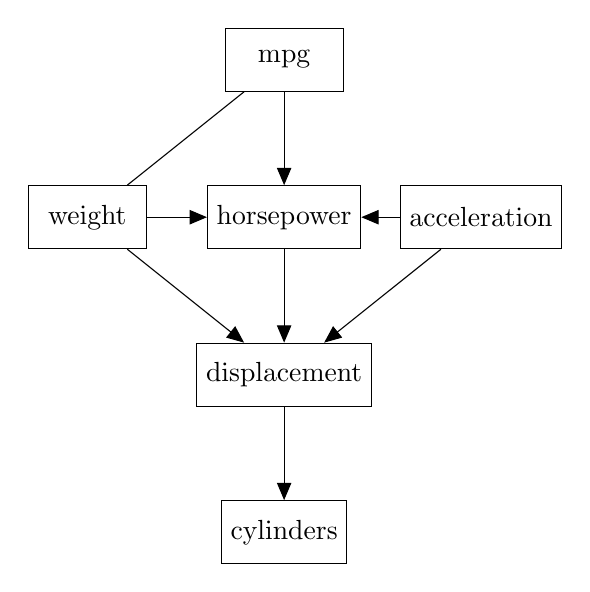
\begin{tikzpicture}[node distance=2cm, every node/.style={draw, rectangle, minimum width=1.5cm, minimum height=0.8cm}, baseline=(mpg.base)]
            % Nodes
            \node (mpg) at (2.5,6) {mpg};
            \node (weight) at (0,4) {weight};
            \node (acceleration) at (5,4) {acceleration};
            \node (horsepower) at (2.5,4) {horsepower};
            \node (displacement) at (2.5,2) {displacement};
            \node (cylinders) at (2.5,0) {cylinders};

            % Edges
            \draw[-] (mpg) -- (weight);
            \draw[->] (mpg) -- (horsepower);
            \draw[->] (horsepower) -- (displacement);
            \draw[->] (displacement) -- (cylinders);
            \draw[->] (acceleration) -- (horsepower);
            \draw[->] (acceleration) -- (displacement);
            \draw[->] (weight) -- (horsepower);
            \draw[->] (weight) -- (displacement);
        \end{tikzpicture}
        \caption{Graph if we lay more emphasis on the test that says that horsepower \textit{is} in the conditioning set yielding that mpg and displacement are independent and \textit{do not} orient the unshielded triple as a collider.}
    \end{subfigure}
    \hfill
    % Second subfigure
    \begin{subfigure}{0.45\textwidth}
        \centering
        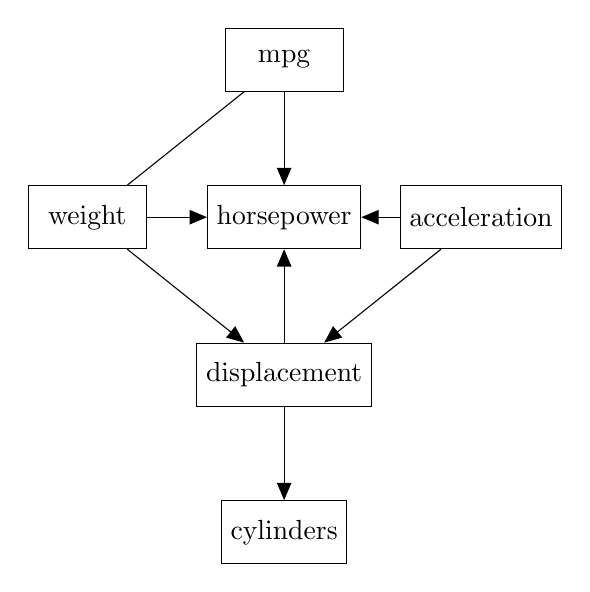
\begin{tikzpicture}[node distance=2cm, every node/.style={draw, rectangle, minimum width=1.5cm, minimum height=0.8cm}, baseline=(mpg.base)]
            % Nodes
            \node (mpg) at (2.5,6) {mpg};
            \node (weight) at (0,4) {weight};
            \node (acceleration) at (5,4) {acceleration};
            \node (horsepower) at (2.5,4) {horsepower};
            \node (displacement) at (2.5,2) {displacement};
            \node (cylinders) at (2.5,0) {cylinders};

            % Edges (only one difference)
            \draw[-] (mpg) -- (weight);
            \draw[->] (mpg) -- (horsepower);
            \draw[->] (displacement) -- (horsepower); % Changed direction
            \draw[->] (displacement) -- (cylinders);
            \draw[->] (acceleration) -- (horsepower);
            \draw[->] (acceleration) -- (displacement);
            \draw[->] (weight) -- (horsepower);
            \draw[->] (weight) -- (displacement);
        \end{tikzpicture}
        \caption{Graph if we lay more emphasis on the test that says that horsepower is \textit{not} in the conditioning set yielding that mpg and displacement are independent and \textit{do} orient the unshielded triple as a collider.}
    \end{subfigure}

    \caption{Comparison of output graphs of PC on auto mpg data after ambiguity resolution.}
    \label{fig:auto_mpg}
\end{figure}

\begin{table}[h]
    \centering
    \begin{tabular}{l c c}
        \toprule
         & \textbf{Resolve as collider} & \textbf{Resolve as non-collider} \\
        \midrule
        Standard Total Coherency Score & 0.9174 & 0.9174 \\
        Standard Markov Coherency Score & 0.9504 & 0.9669 \\
        Standard Faithfulness Coherency Score & 0.9669 & 0.9504 \\
        Conditioning Set Size Adjusted Total Coherency Score & 0.8895 & 0.9004 \\
        Conditioning Set Size Adjusted Markov Coherency Score & 0.9185 & 0.9358 \\
        Conditioning Set Size Adjusted Faithfulness Coherency Score & 0.9709 & 0.9646 \\
        Number of Orientation Conflicts & 0 & 0 \\
        \bottomrule
    \end{tabular}
    \caption{Coherency scores for PC on auto mpg data with the two possible ambiguity resolutions.}
    \label{tab:auto_mpg_coherency_long_version_for_appendix}
\end{table}

\textbf{Toy Models.} It is interesting to analyze small sample properties for different configurations of well-known causal structures. It can show us from which sample size the true causal graph or a coherent but erroneous result is discovered. In combination with comparing the output graphs with the known ground truth––the causal graph of SCM generating the data––we can evaluate which causal structures are correctly discovered and from which sample size the result is almost always correct. This provides a foundation for robustness tests and finite sample analysis. We start with one of the simplest possible models. We round the results and their standard deviation (in brackets) to three decimal places.

\begin{figure}[h]
    \centering
    \begin{subfigure}{0.45\textwidth}
        \centering
        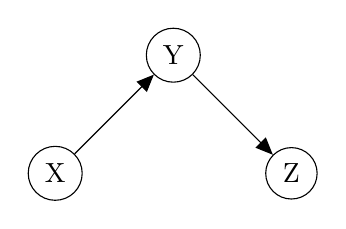
\begin{tikzpicture}[node distance=2cm, every node/.style={draw, circle}, baseline=(y.base)]
            \node (x) at (0,0) {X};
            \node (z) at (3,0) {Z};
            \node (y) at (1.5,1.5) {Y};
            
            \draw[->] (x) -- (y);
            \draw[->] (y) -- (z);
        \end{tikzpicture}
        \caption{The causal graph $\cG_{\text{true}}$ of the data generating SCM.}
    \end{subfigure}
    \hfill
    \begin{subfigure}{0.45\textwidth}
        \centering
        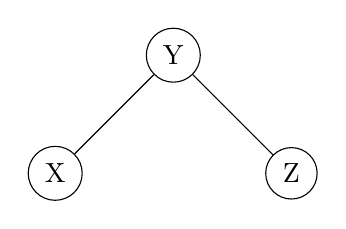
\begin{tikzpicture}[node distance=2cm, every node/.style={draw, circle}, baseline=(y.base)]
            \node (x) at (0,0) {X};
            \node (z) at (3,0) {Z};
            \node (y) at (1.5,1.5) {Y};
            
            \draw[-] (x) -- (y);
            \draw[-] (y) -- (z);
        \end{tikzpicture}
        \caption{Correct result: $\cG_{\text{out}}$ is Markov equivalent to $\cG_{\text{true}}$.}
    \end{subfigure}
    
    \vspace{0.5cm} % Space between rows

    \begin{subfigure}{0.45\textwidth}
        \centering
        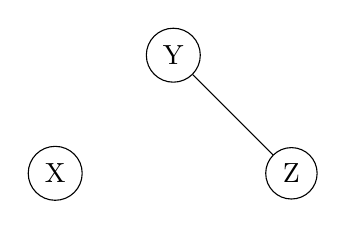
\begin{tikzpicture}[node distance=2cm, every node/.style={draw, circle}, baseline=(y.base)]
            \node (x) at (0,0) {X};
            \node (z) at (3,0) {Z};
            \node (y) at (1.5,1.5) {Y};
            
            \draw[-] (y) -- (z);
        \end{tikzpicture}
        \caption{Markov incoherent tuples in $\cG_{\text{out}}$ due to large effects, e.g. $(X,Z,\emptyset)$.}
    \end{subfigure}
    \hfill
    \begin{subfigure}{0.45\textwidth}
        \centering
        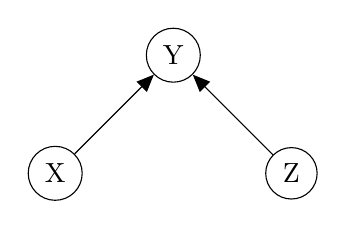
\begin{tikzpicture}[node distance=2cm, every node/.style={draw, circle}, baseline=(y.base)]
            \node (x) at (0,0) {X};
            \node (z) at (3,0) {Z};
            \node (y) at (1.5,1.5) {Y};
            
            \draw[->] (x) -- (y);
            \draw[->] (z) -- (y);
        \end{tikzpicture}
        \caption{Undetectable erroneous result due to effects much smaller than one.}
    \end{subfigure}
    
    \caption{Three output graphs after performing PC on data generated by the SCM in (a) with different effect sizes.}
    \label{fig:mediated_effect}
\end{figure}

\begin{model}[Mediated Effect (three nodes)] \label{model:mediated_effect}
    Consider the following SCM for a constant $c \in \mathbb{R}$:
    \begin{align*}
        X=\eta_{X}, \quad Y=cX+\eta_{Y}, \quad Z=cY+\eta_{Z},
    \end{align*}
    where $\eta_{X}, \eta_{y}, \eta_{Z} \sim \mathbb{N}(0,1)$ are independent exogenous noise variables. This is the model for a simple mediated effect from $X$ to $Z$. We now simulate data from this SCM for different effect strengths $c$, run the PC algorithm and compute the scores (in particular, the standard total, faithfulness and Markov coherency score) for the results. We do so for different sample sizes and average over 100 repetitions for each sample size. The resulting graphs are shown in Figure \ref{fig:mediated_effect}. The average scores are shown in Table \ref{tab:mediated_effect_02} for $c=0.2$ (most simulations yield the graph in Figure \ref{fig:mediated_effect} (d) as the output graph), Table \ref{tab:mediated_effect_1} (most simulations yield the graph in Figure \ref{fig:mediated_effect} (b) as the output graph) and Table \ref{tab:med_effect_four_nodes_10} (simulations with smaller samples often yield the graph in Figure \ref{fig:mediated_effect} (c) as the output, with increasing sample size (b) becomes predominant).
\end{model}

\begin{model}[Mediated Effect (four nodes)] \label{model:mediated_effect_four nodes}
    Consider the following SCM for a constant $c \in \mathbb{R}$ and one more node than in Model \ref{model:mediated_effect}:
    \begin{align*}
        X=\eta_{X}, \quad Y=cX+\eta_{Y}, \quad Z=cY+\eta_{Z}, \quad W=cW+\eta_{W},
    \end{align*}
    where $\eta_{X}, \eta_{y}, \eta_{Z}, \eta_{W} \sim \mathbb{N}(0,1)$ are independent exogenous noise variables. This is the model for a mediated effect from $X$ to $W$ with two mediators. Again, we simulate data from this SCM for different effect strengths $c$, run the PC algorithm and compute the scores (in particular, the standard total, faithfulness and Markov coherency score) for the results. We do so for different sample sizes and average over 100 repetitions for each sample size. The tables show while a very small effect strength of $c=0.2$ leads to a coherent erroneous result for three nodes, see Figure \ref{fig:mediated_effect} (d), the erroneous result becomes detectable for four nodes.
\end{model}

\begin{table}[h]
\centering
\caption{Mediated Effect (Model \ref{model:mediated_effect}) with $c=0.2$}\label{tab:mediated_effect_02}\begin{tabular}{ccccc}
\toprule % from booktabs package
\bfseries & \bfseries 50 & \bfseries 100 & \bfseries 1000 & \bfseries 10000 \\ 
\midrule % from booktabs package
Total & 0.997 (0.033)  & 0.993 (0.047)  & 1.0 (0.0)  & 1.0 (0.0)  \\ 
Faithfulness & 1.0 (0.0)  & 1.0 (0.0)  & 1.0 (0.0)  & 1.0 (0.0)  \\ 
Markov & 0.997 (0.033)  & 0.993 (0.047)  & 1.0 (0.0)  & 1.0 (0.0)  \\ 
Orientation Conflicts & 0.0 & 0.0 & 0.0 & 0.0 \\ 
\bottomrule % from booktabs package
\end{tabular}
\end{table}
% \begin{table}
% \centering
% \caption{Mediated Effect (Model \ref{model:mediated_effect}) with $c=0.5$}\label{tab:mediated_effect_05}\begin{tabular}{ccccc}
% \toprule % from booktabs package
% \bfseries & \bfseries 50 & \bfseries 100 & \bfseries 1000 & \bfseries 10000 \\ 
% \midrule % from booktabs package
% Total & 0.983 (0.073)  & 1.0 (0.0)  & 1.0 (0.0)  & 1.0 (0.0)  \\ 
% Faithfulness & 1.0 (0.0)  & 1.0 (0.0)  & 1.0 (0.0)  & 1.0 (0.0)  \\ 
% Markov & 0.983 (0.073)  & 1.0 (0.0)  & 1.0 (0.0)  & 1.0 (0.0)  \\ 
% Orientation Conflicts & 0.0 & 0.0 & 0.0 & 0.0 \\ 
% \bottomrule % from booktabs package
% \end{tabular}
% \end{table}
\begin{table}[h]
\centering
\caption{Mediated Effect (Model \ref{model:mediated_effect}) with $c=1$}\label{tab:mediated_effect_1}\begin{tabular}{ccccc}
\toprule % from booktabs package
\bfseries & \bfseries 50 & \bfseries 100 & \bfseries 1000 & \bfseries 10000 \\ 
\midrule % from booktabs package
Total & 0.99 (0.057)  & 1.0 (0.0)  & 1.0 (0.0)  & 1.0 (0.0)  \\ 
Faithfulness & 1.0 (0.0)  & 1.0 (0.0)  & 1.0 (0.0)  & 1.0 (0.0)  \\ 
Markov & 0.99 (0.057)  & 1.0 (0.0)  & 1.0 (0.0)  & 1.0 (0.0)  \\ 
Orientation Conflicts & 0.0 & 0.0 & 0.0 & 0.0 \\ 
\bottomrule % from booktabs package
\end{tabular}
\end{table}
% \begin{table}
% \centering
% \caption{Mediated Effect (Model \ref{model:mediated_effect}) with $c=5$}\label{tab:mediated_effect_5}\begin{tabular}{ccccc}
% \toprule % from booktabs package
% \bfseries & \bfseries 50 & \bfseries 100 & \bfseries 1000 & \bfseries 10000 \\ 
% \midrule % from booktabs package
% Total & 0.75 (0.144)  & 0.85 (0.166)  & 1.0 (0.0)  & 1.0 (0.0)  \\ 
% Faithfulness & 1.0 (0.0)  & 1.0 (0.0)  & 1.0 (0.0)  & 1.0 (0.0)  \\ 
% Markov & 0.75 (0.144)  & 0.85 (0.166)  & 1.0 (0.0)  & 1.0 (0.0)  \\ 
% Orientation Conflicts & 0.0 & 0.0 & 0.0 & 0.0 \\ 
% \bottomrule % from booktabs package
% \end{tabular}
% \end{table}
\begin{table}[h]
\centering
\caption{Mediated Effect (Model \ref{model:mediated_effect}) with $c=10$}\label{tab:mediated_effect_10}\begin{tabular}{ccccc}
\toprule % from booktabs package
\bfseries & \bfseries 50 & \bfseries 100 & \bfseries 1000 & \bfseries 10000 \\ 
\midrule % from booktabs package
Total & 0.703 (0.104)  & 0.74 (0.138)  & 0.973 (0.09)  & 1.0 (0.0)  \\ 
Faithfulness & 1.0 (0.0)  & 1.0 (0.0)  & 1.0 (0.0)  & 1.0 (0.0)  \\ 
Markov & 0.703 (0.104)  & 0.74 (0.138)  & 0.973 (0.09)  & 1.0 (0.0)  \\ 
Orientation Conflicts & 0.0 & 0.0 & 0.0 & 0.0 \\ 
\bottomrule % from booktabs package
\end{tabular}
\end{table}

\begin{table}[h]
\centering
\caption{Mediated Effect from Model \ref{model:mediated_effect_four nodes}, $c=0.2$}\label{tab:med_effect_four_nodes_02}\begin{tabular}{ccccc}
\toprule % from booktabs package
\bfseries & \bfseries 50 & \bfseries 100 & \bfseries 1000 & \bfseries 10000 \\ 
\midrule % from booktabs package
Total & 0.988 (0.051)  & 0.976 (0.061)  & 0.906 (0.079)  & 0.923 (0.028)  \\ 
Faithfulness & 0.993 (0.033)  & 0.98 (0.054)  & 0.906 (0.079)  & 0.924 (0.025)  \\ 
Markov & 0.994 (0.04)  & 0.996 (0.031)  & 1.0 (0.0)  & 0.999 (0.011)  \\ 
Orientation Conflicts & 0.04 & 0.15 & 0.7 & 0.02 \\ 
\bottomrule % from booktabs package
\end{tabular}
\end{table}
\begin{table}[h]
\centering
\caption{Mediated Effect from Model \ref{model:mediated_effect_four nodes}, $c=1$}\label{tab:med_effect_four_nodes_1}\begin{tabular}{ccccc}
\toprule % from booktabs package
\bfseries & \bfseries 50 & \bfseries 100 & \bfseries 1000 & \bfseries 10000 \\ 
\midrule % from booktabs package
Total & 0.922 (0.098)  & 0.966 (0.069)  & 0.986 (0.035)  & 0.984 (0.039)  \\ 
Faithfulness & 0.966 (0.051)  & 0.984 (0.043)  & 0.996 (0.024)  & 0.99 (0.034)  \\ 
Markov & 0.957 (0.058)  & 0.982 (0.037)  & 0.99 (0.025)  & 0.994 (0.019)  \\ 
Orientation Conflicts & 0.01 & 0.0 & 0.0 & 0.02 \\ 
\bottomrule % from booktabs package
\end{tabular}
\end{table}
\begin{table}[h]
\centering
\caption{Mediated Effect from Model \ref{model:mediated_effect_four nodes}, $c=10$}\label{tab:med_effect_four_nodes_10}\begin{tabular}{ccccc}
\toprule % from booktabs package
\bfseries & \bfseries 50 & \bfseries 100 & \bfseries 1000 & \bfseries 10000 \\ 
\midrule % from booktabs package
Total & 0.637 (0.08)  & 0.642 (0.083)  & 0.774 (0.068)  & 0.805 (0.071)  \\ 
Faithfulness & 1.0 (0.0)  & 0.997 (0.019)  & 0.916 (0.05)  & 0.901 (0.041)  \\ 
Markov & 0.637 (0.08)  & 0.645 (0.09)  & 0.858 (0.089)  & 0.905 (0.036)  \\ 
Orientation Conflicts & 0.0 & 0.0 & 0.0 & 0.0 \\ 
\bottomrule % from booktabs package
\end{tabular}
\end{table}

\begin{model}[Causal Insufficiency] \label{model:causal_insufficiency}
        Consider the following SCM:
    \begin{align*}
    U_1&=\eta_{U_1}, &U_2&=\eta_{U_2}, &U_3&=\eta_{U_3}, &U_4&=\eta_{U_4} \\
        X&=U_1+U_2+\eta_{X}, &Y&=U_2+U_3+\eta_{Y}, &Z&=U_3+U_4+\eta_{Z}, &V&=U_4+U_1+\eta_{V}.
    \end{align*}
    where $\eta_{X}, \eta_{y}, \eta_{Z}, \eta_{V}, \eta_{U_1}, \eta_{U_2}, \eta_{U_3}, \eta_{U_4} \sim \mathbb{N}(0,1)$ are independent exogenous noise variables and $U_1,U_2,U_3,U_4$ unobserved. We run the PC algorithm on the observed variables and note that there is a structural assumption violation (error code E2), in particular, a causal insufficiency. We note that for the detectable faithfulness violation discussed in Section \ref{sec:experiments}, the score is almost constant between sample sizes and detects the incoherency. For an undetectable causal insufficiency, see Example \ref{ex:causal_insufficiency_undetectable}.
\end{model}

\begin{figure}[h]
    \centering
    % First row of subfigures
    \begin{subfigure}{0.45\textwidth}
        \centering
        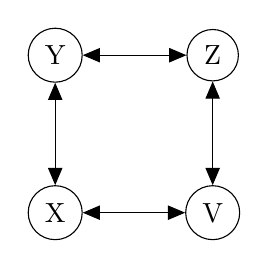
\begin{tikzpicture}[node distance=2cm, every node/.style={draw, circle}, baseline=(y.base)]
            % Nodes
            \node (x) at (0,0) {X};
            \node (y) at (0,2) {Y};
            \node (z) at (2,2) {Z};
            \node (w) at (2,0) {V};

            % Edges
            \draw[<->] (x) -- (y);
            \draw[<->] (y) -- (z);
            \draw[<->] (z) -- (w);
            \draw[<->] (w) -- (x);
        \end{tikzpicture}
        \caption{The causal graph $\cG_{\text{true}}$ of the data generating SCM.}
    \end{subfigure}
    \hfill
    \begin{subfigure}{0.45\textwidth}
        \centering
        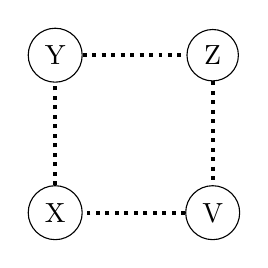
\begin{tikzpicture}[node distance=2cm, every node/.style={draw, circle}, baseline=(y.base)]
            % Nodes
            \node (x) at (0,0) {X};
            \node (y) at (0,2) {Y};
            \node (z) at (2,2) {Z};
            \node (w) at (2,0) {V};

            % Thicker dotted edges
            \draw[dotted, line width=0.5mm] (x) -- (y);
            \draw[dotted, line width=0.5mm] (y) -- (z);
            \draw[dotted, line width=0.5mm] (z) -- (w);
            \draw[dotted, line width=0.5mm] (w) -- (x);
        \end{tikzpicture}
        \caption{Orientation conflicts on all edges in $\cG_{\text{out}}$ after applying PC.}
    \end{subfigure}
    
    \vspace{0.5cm} % Space between rows

    % Second row of subfigures
    \begin{subfigure}{0.45\textwidth}
        \centering
        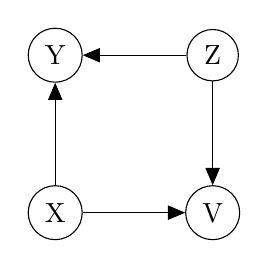
\begin{tikzpicture}[node distance=2cm, every node/.style={draw, circle}, baseline=(y.base)]
            % Nodes
            \node (x) at (0,0) {X};
            \node (y) at (0,2) {Y};
            \node (z) at (2,2) {Z};
            \node (w) at (2,0) {V};

            % Directed edges
            \draw[->] (x) -- (y);
            \draw[->] (z) -- (y);
            \draw[->] (z) -- (w);
            \draw[->] (x) -- (w);
        \end{tikzpicture}
        \caption{The graph $\cG_{\text{out}}$ after applying a conflict resolution strategy: faithfulness incoherent tuple $(Y,V,\emptyset)$.}
    \end{subfigure}
    \hfill
    \begin{subfigure}{0.45\textwidth}
        \centering
        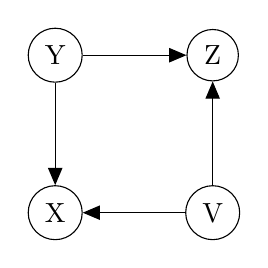
\begin{tikzpicture}[node distance=2cm, every node/.style={draw, circle}, baseline=(y.base)]
            % Nodes
            \node (x) at (0,0) {X};
            \node (y) at (0,2) {Y};
            \node (z) at (2,2) {Z};
            \node (w) at (2,0) {V};

            % Directed edges in different orientation
            \draw[->] (y) -- (x);
            \draw[->] (y) -- (z);
            \draw[->] (w) -- (z);
            \draw[->] (w) -- (x);
        \end{tikzpicture}
        \caption{The graph $\cG_{\text{out}}$ after applying another conflict resolution strategy: faithfulness incoherent tuple $(X,Z,\emptyset)$.}
    \end{subfigure}
    
    \caption{Comparison of outputs of PC on causally insufficient data with and without conflict resolution.}
    \label{fig:causal_graph_comparison}
\end{figure}
\begin{table}[h]
\centering
\caption{Causal Insufficiency Model \ref{model:causal_insufficiency}}\label{tab:causal_insufficiency}\begin{tabular}{ccccc}
\toprule % from booktabs package
\bfseries & \bfseries 50 & \bfseries 100 & \bfseries 1000 & \bfseries 10000 \\ 
\midrule % from booktabs package
Total & 0.891 (0.084)  & 0.846 (0.044)  & 0.843 (0.033)  & 0.849 (0.039)  \\ 
Faithfulness & 0.896 (0.08)  & 0.846 (0.044)  & 0.843 (0.033)  & 0.849 (0.039)  \\ 
Markov & 0.995 (0.037)  & 1.0 (0.0)  & 1.0 (0.0)  & 1.0 (0.0)  \\ 
Orientation Conflicts & 1.27 & 3.14 & 3.58 & 3.44 \\ 
\bottomrule % from booktabs package
\end{tabular}
\end{table}

\begin{model}[Classical Five Node Toy Model] \label{model:five_node_classical}
   Consider the following SCM:
\begin{align*}
   X &= \eta_{X}, &Y &= \eta_{Y}, &Z &= cX+cY+\eta_{Z} \\
    W &= cZ + \eta_{W}, &V &= cZ +\eta_{V},
\end{align*}
where $\eta_{X},\eta_{Y},\eta_{Z},\eta_{V},\eta_{W} \sim \mathcal{N}(0,1)$ are independent, exogenous noise terms.
\end{model}
\begin{table}[h]
\centering
\caption{Five Node Model (Model \ref{model:five_node_classical}) $c=0.2$}\label{tab:five_nide_classical_02}\begin{tabular}{ccccc}
\toprule % from booktabs package
\bfseries & \bfseries 50 & \bfseries 100 & \bfseries 1000 & \bfseries 10000 \\ 
\midrule % from booktabs package
Total & 0.981 (0.054)  & 0.959 (0.055)  & 0.938 (0.053)  & 0.99 (0.021)  \\ 
Faithfulness & 0.992 (0.026)  & 0.988 (0.03)  & 0.969 (0.027)  & 0.991 (0.018)  \\ 
Markov & 0.988 (0.047)  & 0.971 (0.052)  & 0.969 (0.027)  & 0.999 (0.006)  \\ 
Orientation Conflicts & 0.1 & 0.19 & 0.0 & 0.0 \\ 
\bottomrule % from booktabs package
\end{tabular}
\end{table}
\begin{table}[h]
\centering
\caption{Five Node Model (Model \ref{model:five_node_classical}) $c=1$}\label{tab:five_nide_classical_1}\begin{tabular}{ccccc}
\toprule % from booktabs package
\bfseries & \bfseries 50 & \bfseries 100 & \bfseries 1000 & \bfseries 10000 \\ 
\midrule % from booktabs package
Total & 0.724 (0.079)  & 0.789 (0.094)  & 0.99 (0.023)  & 0.992 (0.018)  \\ 
Faithfulness & 0.947 (0.043)  & 0.937 (0.034)  & 0.99 (0.023)  & 0.992 (0.018)  \\ 
Markov & 0.777 (0.078)  & 0.852 (0.093)  & 1.0 (0.0)  & 1.0 (0.0)  \\ 
Orientation Conflicts & 0.07 & 0.04 & 0.0 & 0.0 \\ 
\bottomrule % from booktabs package
\end{tabular}
\end{table}
\begin{table}
\centering
\caption{Five Node Model (Model \ref{model:five_node_classical}) $c=10$}\label{tab:five_nide_classical_10}\begin{tabular}{ccccc}
\toprule % from booktabs package
\bfseries & \bfseries 50 & \bfseries 100 & \bfseries 1000 & \bfseries 10000 \\ 
\midrule % from booktabs package
Total & 0.79 (0.044)  & 0.792 (0.036)  & 0.788 (0.042)  & 0.78 (0.04)  \\ 
Faithfulness & 1.0 (0.002)  & 1.0 (0.002)  & 1.0 (0.0)  & 0.996 (0.015)  \\ 
Markov & 0.79 (0.043)  & 0.792 (0.036)  & 0.788 (0.042)  & 0.784 (0.035)  \\ 
Orientation Conflicts & 0.0 & 0.01 & 0.0 & 0.0 \\ 
\bottomrule % from booktabs package
\end{tabular}
\end{table}

Last, we want to give the full version of the table in the main paper corresponding to the model described in Example \ref{ex:unfaithfulness_detectable}.

\begin{table}[h]
\centering
\caption{Faithfulness Violation from Example \ref{ex:unfaithfulness_detectable}}\label{tab:faithfulness_violation_extended_version_appendix}\begin{tabular}{ccccc}
\toprule % from booktabs package
\bfseries & \bfseries 50 & \bfseries 100 & \bfseries 1000 & \bfseries 10000 \\ 
\midrule % from booktabs package
Total & 0.9 (0.056)  & 0.879 (0.038)  & 0.876 (0.03)  & 0.884 (0.041)  \\ 
Faithfulness & 0.945 (0.033)  & 0.938 (0.019)  & 0.936 (0.013)  & 0.939 (0.019)  \\ 
Markov & 0.954 (0.06)  & 0.941 (0.033)  & 0.94 (0.02)  & 0.945 (0.025)  \\ 
Orientation Conflicts & 0.08 & 0.01 & 0.0 & 0.0 \\ 
\bottomrule % from booktabs package
\end{tabular}
\end{table}

\section{Additional Examples} \label{app:additional_examples}

We first present an example that show how the assumptions of additivity in a nonlinear regression-based CI test may not be in line with the assumption of additivity in the underlying data generating mechanism.

\begin{example} \label{ex.gpdc}

Consider the following additive noise data generating mechanism
\begin{align*}
   Z_1 &= \eta_{Z_1}, &Z_2 &= \eta_{Z_2}, &Z_3 &= \eta_{Z_3} \\
    X &= Z_1 \cdot Z_2 + \eta_{X}, &Y &= Z_2 \cdot Z_3 + \eta_{Y},
\end{align*}

with independent, exogenous noise terms$\eta_{Z_1},\eta_{Z_2},\eta_{Z_3},\eta_{X}, \eta_{Y}$. The corresponding causal graph is shown in Figure \ref{fig:additive_model}. Since every structural equation above is expressed in the form $X  = f(\textbf{S})+ \eta_X$, it is tempting to use a test $T$ that evaluates $X \ind Y | \mathbf{S}$ by first regressing $X$ and $Y$ on $\mathbf{S}$ and then testing for independence of the residuals (for instance, GPDC or HSIC). But this example shows that even when $\mathbf{S}^*$ is an additive noise model, the additive noise assumption does not hold for \emph{every tuple $(X,Y,S)\in\cT$} examined in a run of $\cM$. 

In the graph above, we can see that $X \bowtie_{\cG} Y | Z_2$. However, while $X$ (and similarly $Y$) can be expressed as a function of $Z_1$ ($Z_3$) and $Z_2$ with purely additive noise, neither can be expressed as a function of solely $Z_2$ with purely additive noise: for $X$, the parent $Z_1$--which is not in the conditioning set--acts as a multiplicative noise term in the regression of $X$ on $Z_2$. Therefore, even in the infinite sample limit there is no guarantee that a regression-based test will correctly identify the conditional independence $X \ind Y | Z_2$ if the test relies on an assumption of additive noise. When running a method $\cM$ that employs the test $T$, \emph{every causal and non-causal regression executed within} $\cM$ must satisfy those assumptions -- not just the structural equations in the underlying data-generating mechanism.
\end{example}

\begin{figure}[h]
    \centering
        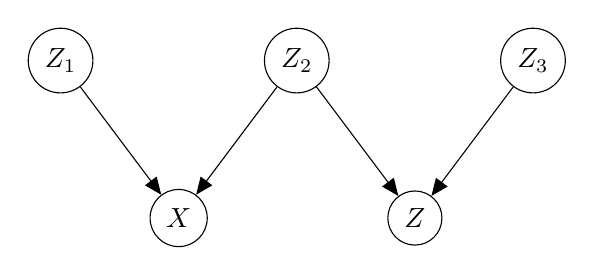
\begin{tikzpicture}[node distance=2cm, every node/.style={draw, circle}, baseline=(y.base)]
            \node (x) at (1.5,0) {$X$};
            \node (y) at (4.5,0) {$Z$};
            \node (z1) at (0,2) {$Z_1$};
            \node (z2) at (3,2) {$Z_2$};
            \node (z3) at (6,2) {$Z_3$};            
            
            \draw[->] (z1) -> (x);
            \draw[->] (z2) -> (x);
            \draw[->] (z2) -> (y);
            \draw[->] (z3) -> (y);
        \end{tikzpicture} 
        \caption{The causal graph $\cG_{\text{true}}$ of the data generating SCM of Example \ref{ex.gpdc} which is correctly discovered by the PC-like method in the infinite sample limit. However, the tuple $(X,Y,\{Z_2\})$ is not guaranteed to be in $\cT^{ind}$ even though clearly $(X,Y,\{Z_2\})\in \cC^{sep}$.}
        \label{fig:additive_model}
\end{figure}

The next example shows that what we call an incoherency is not the same as what is called an inconsistency in \citep{li_constraint-based_2019}.

\begin{example} \label{ex.Markov2}
Consider four variables $W, X,Y,Z$ and assume that the PC-algorithm measures the following during its execution: first, all variables will be judged pairwise dependent (tests with $|\mathbf{S}| = 0$). In the next step, tests with $|\mathbf{S}| = 1$ yield 
\begin{align*}
&W \notind Z | X, \quad W \ind_{(T,\alpha)} Z | Y, \\
&W \ind_{(T,\alpha)} Y | X, \quad X \ind_{(T,\alpha)} Z | Y.    
\end{align*}
All remaining tests with $|\mathbf{S}| = 2$ yield dependence. \\
PC will output the unoriented chain $W-X-Y-Z$, on which $W$ and $Z$ are $d$-separated by $X$, even though $W \notind Z | X$ was measured. Every separating set lies on a path connecting the two variables it separates, i.e. all separating sets are consistent in the sense of \citep{li_constraint-based_2019}.  
\end{example}

The next example shows that a faithfulness violation can lead to an undetectable erroneous result. It is another possible example to illustrate Observation \ref{obs:no_conflicts_but_errors}.

\begin{example} \label{ex:unfaithfulness_undetectable}
    We consider the following ground truth structural causal model:
    \begin{equation*}
        X=\eta_X,\,\,\,\,\,
        Z=X+\eta_Z,\,\,\,\,\,
        Y=2X-2Z+\eta_Y,
    \end{equation*}
    with independent, exogenous noise variables $\eta_X, \eta_Z, \eta_Y \sim \mathcal{N}(0,1)$. The corresponding true causal graph is $\cG_{true}$ in Figure \ref{fig:faithfulness_undetectable}. Note that there is a perfect counteractive mechanism: the direct positive effect of $X$ on $Y$ plus the mediated negative effect of $X$ on $Y$ via $Z$ cancel out, i.e. a faithfulness violation (E1). Assuming no other sources of errors, and choosing the classical PC algorithm as the PC-like method $\cM$, this leads to testing $X$ and $Y$ to be unconditionally independent and all other tuples to be dependent, i.e. $\cT^{ind}=(X,Y,\emptyset)$.
    There is a distribution capturing these independencies and dependencies which is also Markovian to $\cG^{out}$ (F3), see Figure \ref{fig:faithfulness_undetectable}. There are no orientation conflicts and the method has no internal incoherencies (G3). In this case, we have no chance to detect that in fact there was a faithfulness violation and out output is erroneous.
\end{example}

\begin{figure}[h]
    \centering
    \resizebox{.4\textwidth}{!}{ % Scale the entire figure uniformly
        \begin{tabular}{@{}c@{\hspace{1cm}}c@{}} % Added horizontal space between columns
            % First graph: G_true
            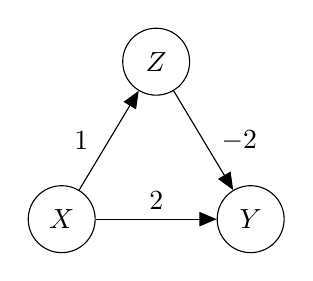
\begin{tikzpicture}[latent/.append style={minimum size=0.85cm}, obs/.append style={minimum size=0.85cm}, det/.append style={minimum size=1.15cm}, wrap/.append style={inner sep=2pt}, on grid]
                % Nodes
                \node[latent] (x) at (0,0) {$X$};
                \node[latent] (y) at (2.4,0) {$Y$};
                \node[latent] (z) at (1.2,2) {$Z$};
                
                % Edges with weights
                \draw[->] (x) -- (y) node[midway, above] {$2$};
                \draw[->] (z) -- (y) node[pos=0.5, right=3pt] {$-2$};
                \draw[->] (x) -- (z) node[pos=0.5, left=4pt] {$1$};
            \end{tikzpicture}
            &
            % Second graph: G_out
            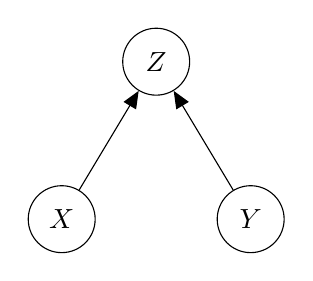
\begin{tikzpicture}[latent/.append style={minimum size=0.85cm}, obs/.append style={minimum size=0.85cm}, det/.append style={minimum size=1.15cm}, wrap/.append style={inner sep=2pt}, on grid]
                % Nodes
                \node[latent] (x) at (0,0) {$X$};
                \node[latent] (y) at (2.4,0) {$Y$};
                \node[latent] (z) at (1.2,2) {$Z$};
                
                % Undirected edges without weights
                \draw[->] (x) -- (z);
                \draw[->] (y) -- (z);
            \end{tikzpicture}
            \\
            $ \cG_{true} $ & $ \cG_{out} $
        \end{tabular}
    }
    \caption{Faithfulness violation leading to a coherent but erroneous result.}
    \label{fig:faithfulness_undetectable}
\end{figure}

\begin{example} \label{ex:causal_insufficiency_undetectable}
    We want to stress that there can also be undetectable causal insufficiencies. Consider the following SCM:
    \begin{align*}
    U_1&=\eta_{U_1}, &U_2&=\eta_{U_2}, &U_3&=\eta_{U_3},\\
        X&=U_1+U_2+\eta_{X}, &Y&=U_2+U_3+\eta_{Y}, &Z&=U_3+U_1+\eta_{Z}.
    \end{align*}
    where $\eta_{X}, \eta_{y}, \eta_{Z}, \eta_{U_1}, \eta_{U_2}, \eta_{U_3} \sim \mathbb{N}(0,1)$ are independent exogenous noise variables and $U_1,U_2,U_3$ unobserved. The resulting graphs are shown in Figure \ref{fig:causal_insufficiency_undetectable}.
\end{example}

\begin{figure}[h]
    \centering
        \resizebox{.4\textwidth}{!}{
        \begin{tabular}{@{}c@{\hspace{1cm}}c@{}} % Added horizontal space between columns
            % First graph: G_true
            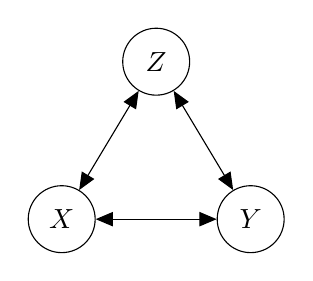
\begin{tikzpicture}[latent/.append style={minimum size=0.85cm}, obs/.append style={minimum size=0.85cm}, det/.append style={minimum size=1.15cm}, wrap/.append style={inner sep=2pt}, on grid]
                % Nodes
                \node[latent] (x) at (0,0) {$X$};
                \node[latent] (y) at (2.4,0) {$Y$};
                \node[latent] (z) at (1.2,2) {$Z$};
                
                % Edges with weights
                \draw[<->] (x) -- (y);
                \draw[<->] (z) -- (y);
                \draw[<->] (x) -- (z);
            \end{tikzpicture}
            &
            % Second graph: G_out
            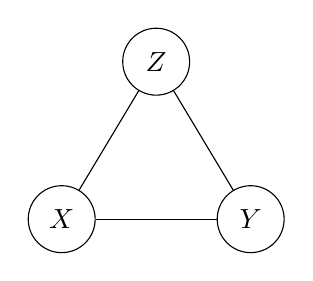
\begin{tikzpicture}[latent/.append style={minimum size=0.85cm}, obs/.append style={minimum size=0.85cm}, det/.append style={minimum size=1.15cm}, wrap/.append style={inner sep=2pt}, on grid]
                % Nodes
                \node[latent] (x) at (0,0) {$X$};
                \node[latent] (y) at (2.4,0) {$Y$};
                \node[latent] (z) at (1.2,2) {$Z$};
                
                % Undirected edges without weights
                \draw[-] (x) -- (z);
                \draw[-] (y) -- (z);
                \draw[-] (x) -- (y);
            \end{tikzpicture}
            \\
            $ \cG_{true} $ & $ \cG_{out} $
        \end{tabular}
        }
    \caption{Causal insufficiency leading to a coherent result.}
    \label{fig:causal_insufficiency_undetectable}
\end{figure}


\end{document}